\documentclass{article}

  % packages
    % basic stuff for rendering math
    \usepackage[letterpaper, top=1in, bottom=1in, left=1in, right=1in]{geometry}
    \usepackage[utf8]{inputenc}
    \usepackage[english]{babel}
    \usepackage{amsmath} 
    \usepackage{amssymb}

    % extra math symbols and utilities
    \usepackage{mathtools}        % for extra stuff like \coloneqq
    \usepackage{mathrsfs}         % for extra stuff like \mathsrc{}
    \usepackage{centernot}        % for the centernot arrow 
    \usepackage{bm}               % for better boldsymbol/mathbf 
    \usepackage{enumitem}         % better control over enumerate, itemize
    \usepackage{hyperref}         % for hypertext linking
    \usepackage{fancyvrb}          % for better verbatim environments
    \usepackage{newverbs}         % for texttt{}
    \usepackage{xcolor}           % for colored text 
    \usepackage{listings}         % to include code
    \usepackage{lstautogobble}    % helper package for code
    \usepackage{parcolumns}       % for side by side columns for two column code
    

    % page layout
    \usepackage{fancyhdr}         % for headers and footers 
    \usepackage{lastpage}         % to include last page number in footer 
    \usepackage{parskip}          % for no indentation and space between paragraphs    
    \usepackage[T1]{fontenc}      % to include \textbackslash
    \usepackage{footnote}
    \usepackage{etoolbox}

    % for custom environments
    \usepackage{tcolorbox}        % for better colored boxes in custom environments
    \tcbuselibrary{breakable}     % to allow tcolorboxes to break across pages

    % figures
    \usepackage{pgfplots}
    \pgfplotsset{compat=1.18}
    \usepackage{float}            % for [H] figure placement
    \usepackage{tikz}
    \usepackage{tikz-cd}
    \usepackage{circuitikz}
    \usetikzlibrary{arrows}
    \usetikzlibrary{positioning}
    \usetikzlibrary{calc}
    \usepackage{graphicx}
    \usepackage{algorithmic}
    \usepackage{caption} 
    \usepackage{subcaption}
    \captionsetup{font=small}

    % for tabular stuff 
    \usepackage{dcolumn}

    \usepackage[nottoc]{tocbibind}
    \pdfsuppresswarningpagegroup=1
    \hfuzz=5.002pt                % ignore overfull hbox badness warnings below this limit

  % New and replaced operators
    \DeclareMathOperator{\Tr}{Tr}
    \DeclareMathOperator{\Sym}{Sym}
    \DeclareMathOperator{\Span}{span}
    \DeclareMathOperator{\std}{std}
    \DeclareMathOperator{\Cov}{Cov}
    \DeclareMathOperator{\Var}{Var}
    \DeclareMathOperator{\Corr}{Corr}
    \DeclareMathOperator{\pos}{pos}
    \DeclareMathOperator*{\argmin}{\arg\!\min}
    \DeclareMathOperator*{\argmax}{\arg\!\max}
    \newcommand{\ket}[1]{\ensuremath{\left|#1\right\rangle}}
    \newcommand{\bra}[1]{\ensuremath{\left\langle#1\right|}}
    \newcommand{\braket}[2]{\langle #1 | #2 \rangle}
    \newcommand{\qed}{\hfill$\blacksquare$}     % I like QED squares to be black

  % Custom Environments
    \newtcolorbox[auto counter, number within=section]{question}[1][]
    {
      colframe = orange!25,
      colback  = orange!10,
      coltitle = orange!20!black,  
      breakable, 
      title = \textbf{Question \thetcbcounter ~(#1)}
    }

    \newtcolorbox[auto counter, number within=section]{exercise}[1][]
    {
      colframe = teal!25,
      colback  = teal!10,
      coltitle = teal!20!black,  
      breakable, 
      title = \textbf{Exercise \thetcbcounter ~(#1)}
    }
    \newtcolorbox[auto counter, number within=section]{solution}[1][]
    {
      colframe = violet!25,
      colback  = violet!10,
      coltitle = violet!20!black,  
      breakable, 
      title = \textbf{Solution \thetcbcounter}
    }
    \newtcolorbox[auto counter, number within=section]{lemma}[1][]
    {
      colframe = red!25,
      colback  = red!10,
      coltitle = red!20!black,  
      breakable, 
      title = \textbf{Lemma \thetcbcounter ~(#1)}
    }
    \newtcolorbox[auto counter, number within=section]{theorem}[1][]
    {
      colframe = red!25,
      colback  = red!10,
      coltitle = red!20!black,  
      breakable, 
      title = \textbf{Theorem \thetcbcounter ~(#1)}
    } 
    \newtcolorbox[auto counter, number within=section]{proposition}[1][]
    {
      colframe = red!25,
      colback  = red!10,
      coltitle = red!20!black,  
      breakable, 
      title = \textbf{Proposition \thetcbcounter ~(#1)}
    } 
    \newtcolorbox[auto counter, number within=section]{corollary}[1][]
    {
      colframe = red!25,
      colback  = red!10,
      coltitle = red!20!black,  
      breakable, 
      title = \textbf{Corollary \thetcbcounter ~(#1)}
    } 
    \newtcolorbox[auto counter, number within=section]{proof}[1][]
    {
      colframe = orange!25,
      colback  = orange!10,
      coltitle = orange!20!black,  
      breakable, 
      title = \textbf{Proof. }
    } 
    \newtcolorbox[auto counter, number within=section]{definition}[1][]
    {
      colframe = yellow!25,
      colback  = yellow!10,
      coltitle = yellow!20!black,  
      breakable, 
      title = \textbf{Definition \thetcbcounter ~(#1)}
    } 
    \newtcolorbox[auto counter, number within=section]{example}[1][]
    {
      colframe = blue!25,
      colback  = blue!10,
      coltitle = blue!20!black,  
      breakable, 
      title = \textbf{Example \thetcbcounter ~(#1)}
    } 
    \newtcolorbox[auto counter, number within=section]{code}[1][]
    {
      colframe = green!25,
      colback  = green!10,
      coltitle = green!20!black,  
      breakable, 
      title = \textbf{Code \thetcbcounter ~(#1)}
    } 
    \newtcolorbox[auto counter, number within=section]{algo}[1][]
    {
      colframe = green!25,
      colback  = green!10,
      coltitle = green!20!black,  
      breakable, 
      title = \textbf{Algorithm \thetcbcounter ~(#1)}
    } 

    \definecolor{dkgreen}{rgb}{0,0.6,0}
    \definecolor{gray}{rgb}{0.5,0.5,0.5}
    \definecolor{mauve}{rgb}{0.58,0,0.82}
    \definecolor{darkblue}{rgb}{0,0,139}
    \definecolor{lightgray}{gray}{0.93}
    \renewcommand{\algorithmiccomment}[1]{\hfill$\triangleright$\textcolor{blue}{#1}}

    % default options for listings (for code)
    \lstset{
      autogobble,
      frame=ltbr,
      language=Python,
      aboveskip=3mm,
      belowskip=3mm,
      showstringspaces=false,
      columns=fullflexible,
      keepspaces=true,
      basicstyle={\small\ttfamily},
      numbers=left,
      firstnumber=1,                        % start line number at 1
      numberstyle=\tiny\color{gray},
      keywordstyle=\color{blue},
      commentstyle=\color{dkgreen},
      stringstyle=\color{mauve},
      backgroundcolor=\color{lightgray}, 
      breaklines=true,                      % break lines
      breakatwhitespace=true,
      tabsize=3, 
      xleftmargin=2em, 
      framexleftmargin=1.5em, 
      stepnumber=1
    }

  % Page style
    \pagestyle{fancy}
    \fancyhead[L]{}
    \fancyhead[C]{Muchang Bahng}
    \fancyhead[R]{Spring 2025} 
    \fancyfoot[C]{\thepage / \pageref{LastPage}}
    \renewcommand{\footrulewidth}{0.4pt}          % the footer line should be 0.4pt wide
    \renewcommand{\thispagestyle}[1]{}  % needed to include headers in title page

\begin{document}

\title{Networks}
\author{Muchang Bahng}
\date{Spring 2025}

\maketitle
\tableofcontents
\pagebreak

\section{The Internet}

  The \textbf{Internet} is a global network of computing devices communicating with each other in some way, whether they're sending emails, downloading files, or sharing websites. The Internet is an \textbf{open network}, which means that any computing device can join as long as they follow the \textbf{protocols} (rules that define how each device must communicate with each other). The internet is powered by many layers of protocols, and to create a global network of computing devices, we need: 
  \begin{enumerate}
      \item \textbf{Wires \& Wireless}: Physical connections between devices, plus protocols for converting electromagnetic signals into binary data. 
      \item \textbf{IP}: A protocol that uniquely identifies devices using IP addresses and provides a routing strategy to send data to a destination IP address. 
      \item \textbf{TCP/UDP}: Protocols that can transport packets of data from one device to another and check for errors along the way. 
      \item \textbf{TLS}: A secure protocol for sending encrypted data so that attackers can't view private information. 
      \item \textbf{HTTP \& DNS}: The protocols powering the World Wide Web
  \end{enumerate}

  \subsection{Computer Networks and Types of Networks}

  \begin{definition}
  A \textbf{computer network} is a group of computers (i.e. computing devices) that use a set of common \textit{communication protocols} over digital interconnections for the purpose of sharing resources located on or provided by the \textit{network nodes}. 

  A \textbf{communication protocol} is a system of rules that allow multiple entities of a communications to transmit information via any kind variation of a physical quantity. The protocol defines the rules, syntax, semantics and synchronization of communication and possible error recovery methods. 
  \end{definition}

  A computer network can be visualized as a connected graph of nodes (which may include personal computers, servers, networking hardware, or other specialised or general-purpose hosts). The \textbf{network topology} is the layout, pattern, or organizational hierarchy of the interconnection of network hosts, in contrast to their physical or geographic location. Common layouts are: 
  \begin{enumerate}
      \item \textbf{Line Network}: All nodes are connected in a line. 
  \begin{center}\resizebox{8cm}{0.64cm}{%
  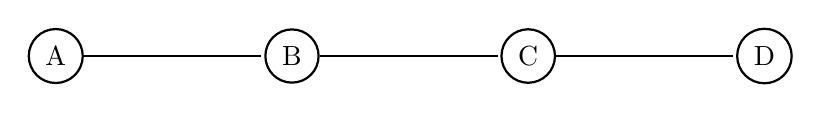
\begin{tikzpicture}[-,>=stealth',shorten >=1pt,auto,node distance=3cm, thick,main node/.style={circle,draw}, every loop/.style={}, scale=0.7]
      \node[main node] (A) {A};
      \node[main node] (B) [right of=A] {B};
      \node[main node] (C) [right of=B] {C};
      \node[main node] (D) [right of=C] {D};
      \path[every node/.style={font=\sffamily\small}]
      (A) edge node {} (B)
      (B) edge node {} (C)
      (C) edge node {} (D);
  \end{tikzpicture}}
  \end{center}
      \item \textbf{Bus Network}: All nodes are connected to a common medium along this medium. 

      \item \textbf{Star Network}: all nodes are connected to a special central node.
  \begin{center}
  \resizebox{3cm}{3cm}{%
  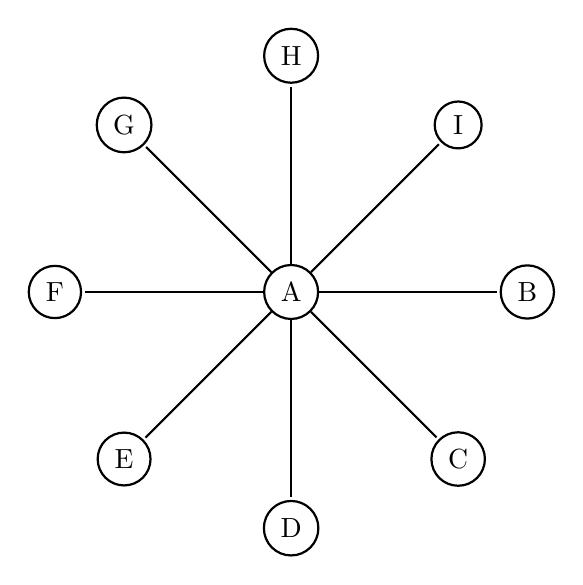
\begin{tikzpicture}[-,>=stealth',shorten >=1pt,auto,node distance=3cm, thick,main node/.style={circle,draw}, every loop/.style={}]
      \node[main node] (A) {A};
      \node[main node] (B) [right of=A] {B};
      \node[main node] (C) [below right of=A] {C};
      \node[main node] (D) [below of=A] {D};
      \node[main node] (E) [below left of=A] {E};
      \node[main node] (F) [left of=A] {F};
      \node[main node] (G) [above left of=A] {G};
      \node[main node] (H) [above of=A] {H};
      \node[main node] (I) [above right of=A] {I};
      \path[every node/.style={font=\sffamily\small}]
      (A) edge node {} (B)
      (A) edge node {} (C)
      (A) edge node {} (D)
      (A) edge node {} (E)
      (A) edge node {} (F)
      (A) edge node {} (G)
      (A) edge node {} (H)
      (A) edge node {} (I);
  \end{tikzpicture}}
  \end{center}
      \item \textbf{Ring Network}: Each node is connected to its left and right neighbour node, such that all nodes are connected and that each node can reach each other node by traversing nodes left- or rightwards.
  \begin{center}
  \resizebox{3cm}{3cm}{%
  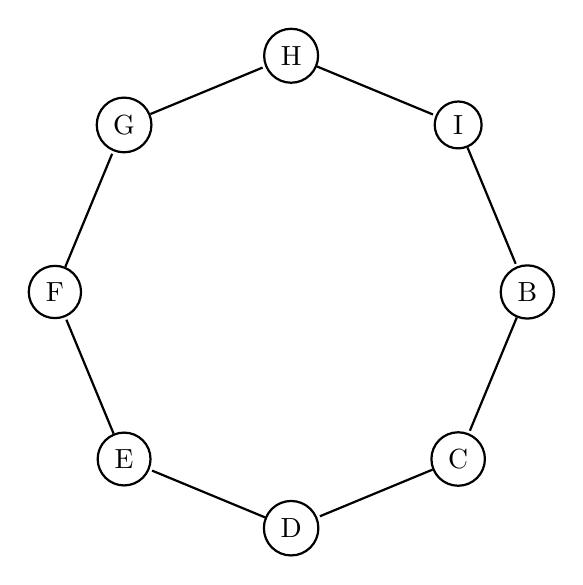
\begin{tikzpicture}[-,>=stealth',shorten >=1pt,auto,node distance=3cm, thick,main node/.style={circle,draw}, every loop/.style={}]
      \node[main node] (A) {A};
      \draw[white, fill=white] (-1,-1) rectangle (1,1);
      \node[main node] (B) [right of=A] {B};
      \node[main node] (C) [below right of=A] {C};
      \node[main node] (D) [below of=A] {D};
      \node[main node] (E) [below left of=A] {E};
      \node[main node] (F) [left of=A] {F};
      \node[main node] (G) [above left of=A] {G};
      \node[main node] (H) [above of=A] {H};
      \node[main node] (I) [above right of=A] {I};
      \path[every node/.style={font=\sffamily\small}]
      (B) edge node {} (C)
      (C) edge node {} (D)
      (D) edge node {} (E)
      (E) edge node {} (F)
      (F) edge node {} (G)
      (G) edge node {} (H)
      (H) edge node {} (I)
      (I) edge node {} (B);
  \end{tikzpicture}}
  \end{center}
      \item \textbf{Mesh Network}: each node is connected to an arbitrary number of neighbours in such a way that there is at least one traversal from any node to any other. 
  \begin{center}
  \resizebox{3.5cm}{3cm}{%
  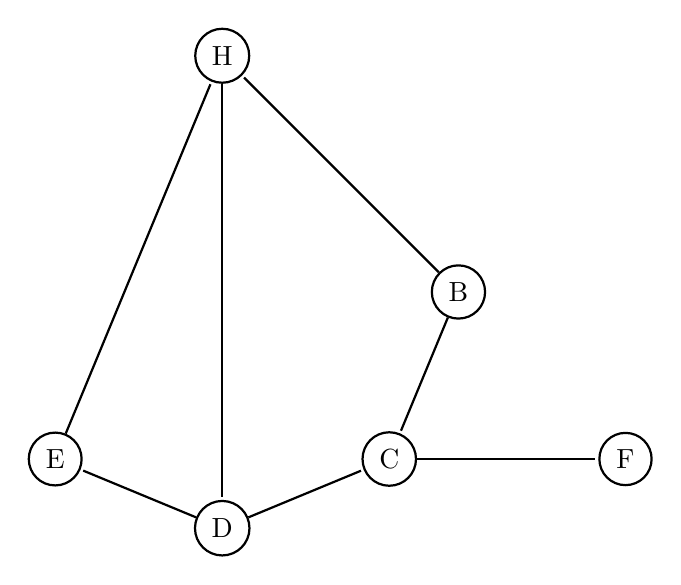
\begin{tikzpicture}[-,>=stealth',shorten >=1pt,auto,node distance=3cm, thick,main node/.style={circle,draw}, every loop/.style={}]
      \node[main node] (A) {A};
      \draw[white, fill=white] (-1,-1) rectangle (1,1);
      \node[main node] (B) [right of=A] {B};
      \node[main node] (C) [below right of=A] {C};
      \node[main node] (D) [below of=A] {D};
      \node[main node] (E) [below left of=A] {E};
      \node[main node] (H) [above of=A] {H};
      \node[main node] (F) [right of=C] {F};
      \path[every node/.style={font=\sffamily\small}]
      (B) edge node {} (C)
      (B) edge node {} (H)
      (D) edge node {} (C)
      (D) edge node {} (E)
      (C) edge node {} (F)
      (E) edge node {} (H)
      (H) edge node {} (D);
  \end{tikzpicture}}
  \end{center}
      \item \textbf{Fully Connected Network}: each node is connected to every other node in the network.
  \begin{center}
  \resizebox{3cm}{3cm}{%
  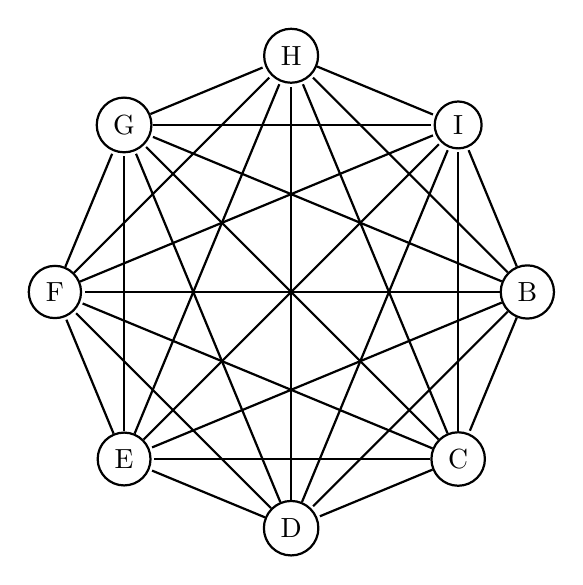
\begin{tikzpicture}[-,>=stealth',shorten >=1pt,auto,node distance=3cm, thick,main node/.style={circle,draw}, every loop/.style={}]
      \node[main node] (A) {A};
      \draw[white, fill=white] (-1,-1) rectangle (1,1);
      \node[main node] (B) [right of=A] {B};
      \node[main node] (C) [below right of=A] {C};
      \node[main node] (D) [below of=A] {D};
      \node[main node] (E) [below left of=A] {E};
      \node[main node] (F) [left of=A] {F};
      \node[main node] (G) [above left of=A] {G};
      \node[main node] (H) [above of=A] {H};
      \node[main node] (I) [above right of=A] {I};
      \path[every node/.style={font=\sffamily\small}]
      (B) edge node {} (C)
      (B) edge node {} (D)
      (B) edge node {} (E)
      (B) edge node {} (F)
      (B) edge node {} (G)
      (B) edge node {} (H)
      (B) edge node {} (I)
      (C) edge node {} (D)
      (C) edge node {} (E)
      (C) edge node {} (F)
      (C) edge node {} (G)
      (C) edge node {} (H)
      (C) edge node {} (I)
      (D) edge node {} (E)
      (D) edge node {} (F)
      (D) edge node {} (G)
      (D) edge node {} (H)
      (D) edge node {} (I)
      (E) edge node {} (F)
      (E) edge node {} (G)
      (E) edge node {} (H)
      (E) edge node {} (I)
      (F) edge node {} (G)
      (F) edge node {} (H)
      (F) edge node {} (I)
      (G) edge node {} (H)
      (G) edge node {} (I)
      (H) edge node {} (I);
  \end{tikzpicture}}
  \end{center}
      \item \textbf{Tree Network}: nodes are arranged hierarchically.
  \begin{center}
  \resizebox{5cm}{3cm}{%
  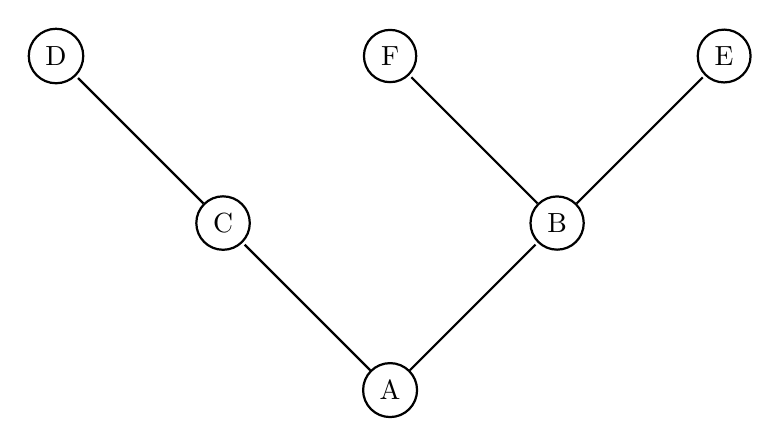
\begin{tikzpicture}[-,>=stealth',shorten >=1pt,auto,node distance=3cm, thick,main node/.style={circle,draw}, every loop/.style={}]
      \node[main node] (A) {A};
      \node[main node] (B) [above right of=A] {B};
      \node[main node] (C) [above left of=A] {C};
      \node[main node] (D) [above left of=C] {D};
      \node[main node] (E) [above right of=B] {E};
      \node[main node] (F) [above left of=B] {F};
      \path[every node/.style={font=\sffamily\small}]
      (A) edge node {} (B)
      (A) edge node {} (C)
      (B) edge node {} (F)
      (B) edge node {} (E)
      (C) edge node {} (D);
  \end{tikzpicture}}
  \end{center}
  \end{enumerate}

  Notice how many of these networks have \textbf{redundancy}: having multiple ways to get from one node to another. That is, when a network path is no longer available, data is still able to reach its destination through another path. Usually, we would like to avoid a \textbf{single point of failure} and construct a \textbf{fault-tolerant} system that can experience failure in its components but still continue operating properly. However, building more connections may be expensive. 

  \begin{example}
  The ARTPANET was the precursor to the Internet, the network where Internet technology was first tested out. It was started in 1969 with four computers connected to each other. 
  \begin{center}\resizebox{5cm}{3cm}{%
  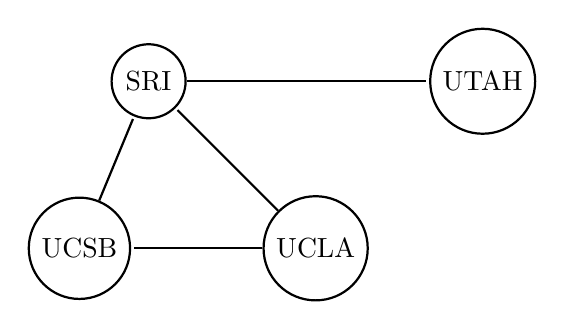
\begin{tikzpicture}[-,>=stealth',shorten >=1pt,auto,node distance=3cm, thick,main node/.style={circle,draw}, every loop/.style={}]
      \node[main node] (UCLA) {UCLA};
      \node[main node] (UCSB) [left of=UCLA] {UCSB};
      \node[main node] (SRI) [above left of=UCLA] {SRI};
      \node[main node] (UTAH) [above right of=UCLA] {UTAH};
      \path[every node/.style={font=\sffamily\small}]
      (UCLA) edge node {} (UCSB)
      (UCLA) edge node {} (SRI)
      (UCSB) edge node {} (SRI)
      (SRI) edge node {} (UTAH);
  \end{tikzpicture}}
  \end{center}
  For example, even if the path between SRI and UCSB is gone, the connections between SRI and UCSB is not lost (since IP packets can travel through UCLA's router). 
  \end{example}

  Because there are multiple paths that a piece of data takes to get from point X to point Y, \textit{routing strategies} are implemented in order to determine the most optimal path.  

  \begin{definition}
  Networks can be categorized as such: 
  \begin{enumerate}
      \item A \textbf{local area network (LAN)} is a computer network that interconnects computers within a limited area. \textit{Ethernet} and \textit{Wi-Fi} are the two most common technologies in use for local area networks. A \textbf{wireless local area network (WLAN)} use radio frequencies to transmit and receive data. 
      \item A \textbf{metropolitan area network (MAN)} is a computer network that interconnects users with computer resources in a geographic region of the size of a metropolitan area. 
      \item In contrast, a \textbf{wide area network (WAN)} not only covers a larger geographic distance, but also generally involves \textit{leased telecommunication circuits} or \textit{data lines} (i.e. a private line between multiple locations provided according to a commercial contract), since no single company owns all the infrastructure across the wide geographic area. It is often composed of many LANs. 
      \item Another type  of network is the \textbf{Data Center Network (DCN)}, a network used in data centers where data must be exchanged with very little delay.
  \end{enumerate}
  \end{definition}

  \subsection{Communication with Line Coding}

  Computers can connect through \textbf{physical} (e.g. cables) or \textbf{wireless} connections. 
  \begin{enumerate}
      \item The \textbf{CAT5 cable} is a \textit{twisted pair (copper) cable} that's designed for use in computer networks. It consists of four twisted pairs of copper wires. These twisted pair cables send data through a network by transmitting pulses of electricity that represent binary data. The information transmission follow the \textbf{Ethernet} standards, which is why twisted pair cables are commonly known as Ethernet cables. Use for both LANs and WANs. They can carry up to 1 Gbps across hundreds of feet, but are susceptible to interference. 
      \item \textbf{Fiber-optic cables} carry light instead of electricity in a fiber coated with plastic layers. The pulses of light represent binary data and also follow the Ethernet standards. They are also capable of transmitting much more data per second that copper cables, and they have the advantage of low transmission loss and immunity to electrical interference. Often used to connect networks across oceans so that data can travel quickly around the world. They can carry up to 26 Tbps acorss 50 miles (but are expensive)
      \item A wireless card inside a computer turns binary data into \textbf{radio waves} and transmits them through the air. However, they do not travel very far (~100 ft in office buildings or up to 1000 ft in an open field). The waves are picked up by a \textit{wireless access point} which converts them from radio waves back into binary data. These access points would be connected to the rest of the network using physical wiring. They can carry up to 1.3 Gbps. 
      \item \textbf{Infrared signals} and \textbf{microwaves} are sometimes used. 
  \end{enumerate}


  In order for the computers to send data into binary, they must convert this data into binary and send them as streams of 1s and 0s in a process called \textbf{line coding}. Furthermore, computers can raise efficiency of each wire by sending changing electric currents through a single wire. For example, rather than using three wires to encode $\texttt{101}$ as 
  \begin{center}
  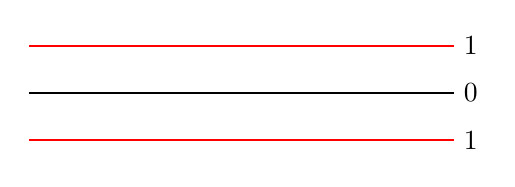
\begin{tikzpicture}[scale=0.6]
      \draw[thick, red] (0,1)--(9,1);
      \draw[thick] (0,0)--(9,0);
      \draw[thick, red] (0,-1)--(9,-1);
      \node[right] at (9,1) {1};
      \node[right] at (9,0) {0}; 
      \node[right] at (9,-1) {1};
  \end{tikzpicture}
  \end{center}
  they send it through a single wire with intervals of $\frac{1}{3}$ seconds
  \begin{center}
  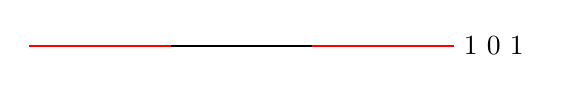
\begin{tikzpicture}[scale=0.6]
      \draw[thick, red] (0,0)--(3,0);
      \draw[thick] (3,0)--(6,0);
      \draw[thick, red] (6,0)--(9,0);
      \node[right] at (9,0) {1 0 1};
  \end{tikzpicture}
  \end{center}
  or even better, at a rate of 1 megabit per second (interval of $0.000001$ seconds)
  \begin{center}
  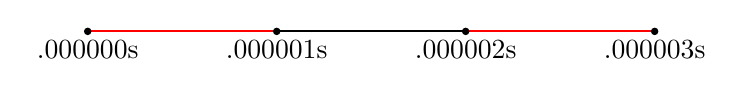
\begin{tikzpicture}[scale=0.8]
      \draw[thick, red] (0,0)--(3,0);
      \draw[thick] (3,0)--(6,0);
      \draw[thick, red] (6,0)--(9,0);
      \draw[fill] (0,0) circle (0.05);
      \draw[fill] (3,0) circle (0.05);
      \draw[fill] (6,0) circle (0.05);
      \draw[fill] (9,0) circle (0.05);
      \node[below] at (0,0) {.000000s};
      \node[below] at (3,0) {.000001s};
      \node[below] at (6,0) {.000002s};
      \node[below] at (9,0) {.000003s};
  \end{tikzpicture}
  \end{center}

  As long as two computers agree on the time period in which the electricity intervals are being sent, they can communicate much more efficiently. In an electrical connection (such as Ethernet), the signal would be a voltage or current. In an optical connection (such as a fiber-optic cable), the signal would be the intensity of light. 

  \begin{definition}
  There are many properties about line coding that are relevant:
  \begin{enumerate}
      \item The \textbf{bit rate} describes the data transfer rate of a connection. It measures the number of bit states that a channel can \textit{transmit} per unit time. It is measured in \textit{bits per second}. We can interpret it as the amount of water flowing through a pipe. 
      
      Bit rate is typically seen in terms of the actual data rate. But for most transmissions, the data represents part of a more complex protocol, which includes bits representing source address, destination address, error detection/correction codes, and other information. This data is called the \textbf{overhead}, while the actual data transferred is called the \textbf{payload}. At times, the overhead may be substantial (up to 20\% to 50\%). 

      \item The \textbf{throughput} is the number of bit states of usable information, that can be successfully \textit{received} over a channel per unit time. Without any channel noise, it is really just the payload. Note that this is an \textit{observed, dynamic parameter} with a fixed and variable loss. It is also known as \textbf{consumed bandwidth} and is measured in \textit{bits per second}. 
      
      \item The \textbf{bandwidth} describes the \textit{maximum} data transfer rate of a connection; that is, the maximum throughput of a communication. It is measured in \textit{bits per second}. We can interpret it as how thick the pipe is (i.e. how much water can flow through it at max). Note that this is different from the bandwidth used in signal processing. 
      
      Data often flows over multiple network connections, which means the connection with the smallest bandwidth (most likely your local connection) acts as a bottleneck. 
      
      \item The \textbf{latency}, or \textbf{ping-rate}, measures the round trip time between the sending of a data message to a computer and the receiving of that message, measured in \textit{milliseconds}. We can interpret it as the speed at which the water is flowing through a pipe. We can check latency by doing
      \begin{lstlisting}
  >>>ping www.google.com
  64 bytes: icmp_seq=0 ttl=115 time=37.868 ms
      \end{lstlisting}
      which outputs a latency time of 37.868ms (to get to $\texttt{www.google.com}$ and back) for sending a data packet of 64 bytes. Note that there is an intrinsic limiting factor to latency: the speed of light, which is approximately 1 foot per nanosecond. In addition to distance, another limiting factor is the congestion in the network and the type of connection. 
  \end{enumerate}
  \end{definition}

  \begin{example}
  Given two computers connected by a wire that is configured to transfer 1000 bits per second, the bit rate would be 1 Kbps. However, if the channel has noise and demands retransmission of 10 bits out of every 1000 of the original transmission, then the throughput would be 990 bps. 

  Furthermore, the Ethernet frame can have as many as 1542 bytes. Say that there are 1500 bytes of payload and an overhead of 42 bytes. Then, the \textbf{protocol efficiency} would would be 
  \[\frac{\text{payload}}{\text{frame size}} = \frac{1500}{1542} = 0.9727 = 97.3\%\]
  \end{example}

  Typically, the actual line rate is stepped up by a factor influenced by the overhead to achieve an actual target net data rate. In One Gigabit Ethernet, the actual line rate is 1.25 Gbits/s to achieve a net payload throughput of 1 Gbit/s. In a 10-Gbit/s Ethernet system, gross data rate equals 10.3125 Gbits/s to achieve a true data rate of 10 Gbits/s. The net data rate also is referred to as the throughput, or payload rate, of effective data rate. 

  Some common units of measurement are: 
  \begin{enumerate}
      \item Mbps, Gbps, Tbps (Mega, Giga, Terabits per second)
      \item MBps, GBps, TBps (Mega, Giga, Terabytes per second)
  \end{enumerate}

  In conclusion, speed is a combination of bandwidth and latency. Even if a computer is on a connection with high bandwidth, its speed of sending and receiving messages will still be limited by the latency of the connection.

  \subsection{Internet Protocol: Addresses and Routing Strategies}
  The \textbf{Internet Protocol (IP)} is one of the core protocols in the layers of the internet. It is used in all Internet communication to handle both addressing and routing. 

  \begin{definition}
  The protocol describes the use of \textbf{IP addresses} to uniquely identify Internet-connected devices (for transmission of data). That is, when a computer sends a message to another computer, it must specify the recipient's IP address and also include its own IP address so that the second computer can reply. There are two versions of the Internet Protocol in use today: 
  \begin{enumerate}
      \item \textbf{IPv4}: The first version ever used on the Internet and having the form of 4 \textit{octets} split by periods in between. 
      \[[0-255].[0-255].[0-255].[0-255]\]
      Even though it presented in decimal, computers store them in binary 
      \[74.125.20.113 \iff 01001011.01111101.00010100.01110001\]
      IPv4 addresses can take $2^{32}$ values, but IPv6 was created for more space.
      \item \textbf{IPv6}: The newer standard (introduced in June 2012) is in the form 
      \[\text{FFFF:FFFF:FFFF:FFFF:FFFF:FFFF:FFFF:FFFF}\]
      with hexadecimal digits (total of ~$3.4 \times 10^{39}$ possible IPv6 values). 
  \end{enumerate}
  \end{definition}

  \begin{definition}
  A \textbf{dynamic IP address} is an IP address that can change. For example, each Internet service provider (ISP) has a range of addresses that they can assign, and they might give you a different one of those addresses each time your computer pops up on the network. Therefore, switching to a different WiFi network will definitely give you a new IP address. 

  Computers that act like servers often have \textbf{static IP addresses}. That makes it easier for computers to quickly send requests to the servers. 
  \end{definition}

  \begin{definition}[Hierarchy of IP Addresses]
  The IP addresses are formatted in an \textit{hierarchical way}. The IPv4 address hierarchy is structured as such: The first few numbers (may or may not be divided by octets) could identify a \textbf{network} administered by an Internet Service Provider. The last numbers, which can also represent \textbf{subnetworks} (subnets), identifies a home computer on that network. For example, if we represent the IP address 141.213.127.13 in binary (of 32 bits)
  \[10001101.11010101.01111111.00001101\]
  the first 16 bits could route to all of UMich, the next two bits could route to a specific UMich department, and the final 14 bits could route to individual computers. 
  \begin{center}
  \begin{tabular}{l|l|l}
      1000110111010101 & 01 & 11111100001101  \\
      \hline
      UMich Network & Medicine department & Lab computer 
  \end{tabular}
  \end{center}
  This hierarchy gives UMich the ability to differentiate between $2^2$ departments and $2^{14} = 16,384$ computers within each department. In general, the ability to create hierarchical levels at any point in the IP address allows for greater flexibility in the size of each level of the hierarchy. 
  \end{definition}

  \subsubsection{LAN vs WAN IP Addresses}
  In fact, your computer is not connected to the internet directly. It is actually in a \textbf{private network}, or a \textit{LAN network}, which uses a private IP address space (supported by both IPv4 and v6). Anything on the inside of your private network is not on the Internet; it is on your LAN, an entirely separate network, with its own address space. Anything on your LAN must have a unique (within the LAN) IP address to participate properly with your local network. Therefore, anyone else who has a LAN is also not part of the internet. Even though none of your devices in your network have a public IP address, the router itself does have a public address. That is, to the outside world, all devices identify their internet activity by the one IP address assigned by your ISP.  

  \begin{definition}
  The IP addresses that are in the private network's space are usually divided up into 3 categories. But as of now, the categories don't mean anything. 
  \begin{enumerate}
      \item \textbf{Class A private range addresses}: 10.0.0.0 - 10.255.255.255 (16,777,216 IPs)
      \item \textbf{Class B private range addresses}: 172.16.0.0 – 172.31.255.255 (1,048,576 IPs)
      \item \textbf{Class C private range addresses}: 192.168.0.0 – 192.168.255.255 (65,536 IPs)
  \end{enumerate}
  Since the private IPv4 address space is relatively small, many private IPv4 networks unavoidably use the same address ranges. This can create a problem when merging such networks, as some addresses may be duplicated for multiple devices. In this case, networks or hosts must be renumbered, often a time-consuming task, or a network address translator must be placed between the networks to translate or masquerade one of the address ranges. 
  \end{definition}

  \begin{definition}[NAT]
  In order for LAN devices to connect to the Internet, their outgoing traffic has the source address changed to match that of the internet/WAN IP address of the router. The router keeps track of this, and makes sure any response traffic gets sent to the right internal machine. This is called \textbf{Network Address Translation (NAT)}. There are generally two types of NAT: 
  \begin{enumerate}
      \item \textbf{Basic, one-to-one NAT}: The simplest type of NAT provides a one-to-one translation of IP addresses. In this type of NAT, only the IP addresses, IP header checksum, and any higher-level checksums that include the IP address are changed. Basic NAT can be used to interconnect two IP networks that have incompatible addressing. 
      \item \textbf{One-to-many NAT}: The majority of network address translators map multiple private hosts to one publicly exposed IP address. In a typical configuration, a local network uses one of the designated private IP address subnets. A router in that network has a private address of that address pace. The router it also connected to the Internet with a \textit{public} address assigned by the ISP. As traffic passes from the local network to the Internet, the source address in each packet is translated on the fly from a private address to the public address. The router tracks basic data about each active connection (particularly the destination address and port). When a reply returns to the router, it uses the connection tracking data it stored during the outbound phase to determine the private address on the internal network to which to forward the reply. 
  \end{enumerate}
  All IP packets have a source IP address and a destination IP address. Typically packets passing from the private network to the public network will have their source address modified, while packets passing from the public network back to the private network will have their destination address modified. To avoid ambiguity in how replies are translated, further modifications to the packets are required, such as TCP or UDP. 
  \end{definition}

  You can find your WAN IP address simply by googling it, since your computer sends a message to the Google computers as soon as it loads $\texttt{google.com}$. 

  \begin{example}
  In my case, my computer's LAN IP address is 192.168.0.8, my phone's LAN IP address is 192.168.0.20, and the public IP address (of the router) is 211.109.203.135. Running $\texttt{whois}$ on my computer and phone's IP addresses reveals nothing much about the LAN one (since it is private anyways and many people have the same one), while the public one (about my router) reveals that it is owned by the ISP SK Broadband Co Ltd. But note that both the LAN and WAN IP addresses can change over time depending on your ISP (and as you restart your device). 

  However, if the cell phone has an active data plan and connected to a local LAN at the same time, it will have a \textit{LAN IP address} and an \textit{IP assigned by the mobile network}. When a browser on the phone fetches a web page, the web server will see the \textit{LAN’s gateway (public) IP address}, so essentially the phone deals with three IP’s at that point. The computer on the other hand will only be assigned a LAN IP address but will also be requesting web pages via the same public IP address. 

  Additionally, moving my computer to another network, say Coffeebay, will change its LAN IP address. As I am writing this in the cafe, the new IP address is now 192.168.0.168. The WAN IP address of the Coffeebay network is 125.132.4.126, with the ISP Korea Telecom (KT) Corp. 
  \end{example}

  The three most popular ISPs in Korea are: 
  \begin{enumerate}
      \item KT Corp. 
      \item LGU
      \item SK Broadband 
  \end{enumerate}
  These ISPs are also called \textbf{broadband providers}. The most popular ones in the USA are:
  \begin{enumerate}
      \item AT\&T Internet Services
      \item Comcast High Speed Internet (aka Xfinity)
      \item Verizon High Speed Internet
      \item Charter Communications (including Spectrum formerly Time Warner Cable)
  \end{enumerate}

  By typing in the correct IP into the browser, going into the administrator interface, and logging in, you can modify the WiFi settings.  

  \subsubsection{Routing IP Packets}
  Since there are physical limitations on how large a message can be when \textit{routing} data between computers, many networking protocols split each message into multiple small \textbf{packets}. 

  \begin{definition}
  Due to physical limitations on how large a message can be sent, the Internet Protocol splits messages into \textbf{IP packets}. Each IP packet contains both a header (20 or 24 bytes long) and data (variable length). 
  \begin{enumerate}
      \item The \textbf{header} includes the following: 
      \begin{center}
      \begin{tabular}{l|l}
          Version/Length, Service Type, Packet Length & 1 byte, 1 byte, 2 bytes \\
          Identification & 2 bytes \\
          DF, MF, Fragment Offset & 2 bytes \\
          Time to Live, Transport & 1 byte, 1 byte \\
          Header Checksum & 2 bytes \\
          Source IP Address & 4 bytes\\
          Destination IP Address & 4 bytes \\
          Options, Padding (optional) & 3 bytes, 1 byte \\
          \hline
          Total & 24 bytes
      \end{tabular}
      \end{center}
      \item The \textbf{data} is the actual content, such as a string of letters or part of a webpage. 
  \end{enumerate}
  These packets hop from router to router towards their destination.
  \end{definition}

  \begin{definition}
  A \textbf{router} is a type of computing device used in computer networks that helps move data packets along. The process of a router receiving and sending a packet is as such: 
  \begin{enumerate}
      \item The packet gets sent to a router, and the router receives it. 
      \item The router looks at the packet's IP header, more specifically the destination IP address. For example, the destination IP address may be $\texttt{91.198.174.192}$. 
      \item The router must now forward the packet, but it may have multiple routers to forward it to. In order to choose the router that is the "closest" to the IP destination, it has a \textbf{forwarding table} that helps it pick the next path based on the destination IP address. The table consists of not IP addresses, but the IP address prefixes. For example, 
      \begin{center}
      \begin{tabular}{l|l}
          IP address prefix & path\\
          \hline
          91.112 & \# 1\\
          91.198 & \# 2 \\
          192.92 & \# 3
      \end{tabular}
      \end{center}
      Since IP addresses are by definition hierarchical, the router only needs to store the prefixes. Once the router locates the most specific row on the table for the destination IP address, it sends the packet along that path. 
      \item This is repeated for the next router. 
      \item When the final router is reached, it should have in its forwarding table the exact IP address prefix. 
      \begin{center}
      \begin{tabular}{l|l}
          IP address prefix & path \\
          \hline
          91.112 & \# 1 \\
          91.198.174.192 & Direct \\
          192.92 & \#2 
      \end{tabular}
      \end{center}
      This router now sends the message to the destination IP address, which may be a personal computer or a server. 
  \end{enumerate}
  \end{definition}

  \begin{definition}
  The \textbf{modem}, short for \textbf{modulator demodulator}, "modulates" the signals going between the LAN and Internet. 
  \end{definition}

  The main difference between the router and the modem is that: 
  \begin{enumerate}
      \item The router crates a network between the computers in your home and routes network traffic between them (through Ethernet cables or wireless connection). Your home router has one connection to the Internet and connections to your private local network. 
      \item The modem serves as a bridge between your local network and the Internet. 
  \end{enumerate}
  Some ISPs offer a modem and router in a single device, which has advantages and disadvantages. 

  Note that there are problems with these packets: 
  \begin{enumerate}
      \item A computer might send multiple messages to a destination, and the destination needs to identify which packets belong to which message.
      \item Packets can arrive out of order. That can happen especially if two packets follow different paths to the destination.
      \item Packets can be corrupted, which means that for some reason, the received data no longer matches the originally sent data.
      \item Packets can be lost due to problems in the physical layer or in routers' forwarding tables.
      \item Similarly, packets might be duplicated due to accidental retransmission of the same packet.
  \end{enumerate}

  However, there are higher level data transport protocols in the Internet protocol stack can deal with these problems, such as the \textit{Transmission Control Protocol (TCP)} and \textit{User Datagram Protocol (UDP)}. 

  \subsection{UDP and TCP}

  The \textbf{User Datagram Protocol (UDP)} is a lightweight data transport protocol that works on top of IP. UDP provides a mechanism to detect corrupt data in packets, but it does not attempt to solve other problems that arise with packets, such as lost or out of order packets. That's why UDP is sometimes known as the \textit{Unreliable Data Protocol}. UDP is simple but fast, at least in comparison to other protocols that work over IP. It's often used for time-sensitive applications (such as real-time video streaming) where speed is more important than accuracy.

  When sending packets using UDP over IP, the data portion of each IP packet is formatted as a \textbf{UDP segment}. 
  \[\text{IP Packet } \implies \text{UDP Segment }\]
  Each UDP segment contains an 8-byte header and variable length data. The first 4 bytes of the UDP header store the \textbf{port numbers} (identification numbers) for the source and destination. The next two bytes store the segment length and the checksum. 
  \begin{center}
  \begin{tabular}{l|l}
      Source port \# & 2 bytes \\
      Destination port \# & 2 bytes \\
      Segment length \# & 2 bytes \\
      Checksum \# & 2 bytes \\
      \hline 
      Total & 8 bytes
  \end{tabular}
  \end{center}

  \begin{definition}
  A networked device can receive messages on different virtual \textbf{ports}. The different ports help distinguish different types of network traffic. 
  \end{definition}

  For example, the following command shows the ports in use: 
  \begin{lstlisting}
  >>> sudo lsof -i -n -P | grep UDP
  launchd       1            root   30u  IPv4 UDP *:137
  launchd       1            root   31u  IPv4 UDP *:138
  mDNSRespo   164  _mdnsresponder    6u  IPv4 UDP *:5353
  mDNSRespo   164  _mdnsresponder    7u  IPv6 UDP *:5353
  rapportd    356          mbahng   12u  IPv4 UDP *:3722
  systemsta   665            root   17u  IPv4 UDP *:*
  netbiosd  14582        _netbios    3u  IPv4 UDP *:137
  netbiosd  14582        _netbios    4u  IPv4 UDP *:138
  \end{lstlisting}
  Each row start with the name of the process that's using the port (one for going in, another for going out) and ends with the protocol and port number. Since each port number is 2 bytes, the maximum port number can be $2^{16} = 65,535$. 

  The \textbf{segment length} stores the length of the the entire UDP segment (including the header). Since the segment length can be represented in 16 bits, the maximum length of the UDP segment can be 65,635 bytes. 

  The \textbf{checksum} is used check for data corruption. It is computed as such. Before sending off the segment, the sender: 
  \begin{enumerate}
      \item Computes the checksum based on the data in the segment (by literally summing up sections of the the binary representation of the data. 
      \item It stores the computed checksum in the field. 
  \end{enumerate}
  Upon receiving the segment, the recipient: 
  \begin{enumerate}
      \item Computes the checksum based on the received segment. 
      \item Compares the checksums to each other. If the checksums aren't equal, it knows that the data was corrupted. 
  \end{enumerate}

  The \textbf{Transmission Control Protocol (TCP)} is a transport protocol that is used on top of IP to ensure reliable transmission of packets. TCP includes mechanisms to solve many of the problems that arise from packet-based messaging, such as lost packets, out of order packets, duplicate packets, and corrupted packets. Since TCP is the protocol used most commonly on top of IP, the Internet protocol stack is sometimes referred to as \textbf{TCP/IP}.  

  When sending packets using TCP/IP, the data portion of each IP packet is formatted as a \textbf{TCP segment}. 
  \[\text{IP Packet (4 bytes)} \implies \text{TCP Segment (variable)}\]
  The TCP header can contain many more fields than the UDP header and can range in size from 20 to 60 bytes, depending no the size of the options field. It does contain the source port number, destination port number, and checksum. 
  \begin{center}
  \begin{tabular}{l|l}
      Source port \# & 2 bytes \\
      Destination port \# & 2 bytes \\
      Sequence number & 4 bytes \\
      Acknowledgement \# & 4 bytes \\
      Offset and Reserved & 10 bits \\
      URG, AFK, PSH, RST, SYN, FIN bits & 6 bits \\
      Window Size & 2 bytes \\
      Checksum & 2 bytes \\
      Urgent pointer & 2 bytes \\
      Options/Padding & 4 bytes \\
      \hline 
      Total & 39 bytes
  \end{tabular}
  \end{center}

  The process of transmitting a packet with TCP/IP is as such:
  \begin{enumerate}
      \item Two computers first establish a connection through a \textbf{three-way handshake}. Computer 1 sends a packet with the SYN bit set to 1. Then computer 2 sends back a packet with the ACK bit set to 1 plus the SYN bit set to 1. The first computer replies back with ACK=1. (Note that the SYN and ACK bits are part of the TCP header) The three packets involved in the three-way handshake do not typically include any data. Once the computers are done with the handshake, they're ready to receive packets containing actual data.
      \item When a packet of data is sent over TCP, the recipient must always acknowledge what they received in the following way: Computer 1 sends a packet with data and a sequence number. Computer 2 acknowledges it by setting the ACK bit and increasing the acknowledgement number by the length of the received data (note that both numbers are also part of the TCP header). It is easy to see how these two numbers help the computers keep track of which data was successfully received, which data was lost, and which data was accidentally sent twice. 
      \item To close the connection, computer 1 initiates it by sending a packet with the FIN bit set to 1. Computer 2 replies with an ACK and another FIN. After one more ACK from computer 1, the connection is closed. 
  \end{enumerate}

  However, some problems can occur. TCP connections can detect lost packets using a timeout. After sending off a packet, the sender starts a timer and puts the packet in a retransmission queue. If the timer runs out and the sender has not yet received an ACK from the recipient, it sends the packet again. The retransmission may lead to the recipient receiving duplicate packets, if a packet was not actually lost but just very slow to arrive or be acknowledged (which happens when the packet takes a slower route through the Internet). If so, the recipient can simply discard duplicate packets. 

  TCP connections can also detect out of order packets by using the sequence and acknowledgement numbers. When the recipient sees a higher sequence number than what they have acknowledged so far, they will know that they are missing at least one packet in between.

  \subsection{Domain Name System (DNS), Hypertext Transfer Protocol (HTTP)}

  \begin{definition}
  The \textbf{world wide web}, or \textbf{the web}, is a network of webpages, programs, and files that are accessible via URLs. It is a subsection of the Internet. A web browser loads a webpage using various protocols: 
  \begin{enumerate}
      \item \textbf{Domain Name System (DNS) protocol} for converting domain names into IP addresses. 
      \item \textbf{HyperText Transfer Protocol (HTTP)} to request the webpage contents from that IP address. 
      \item \textbf{Transport Layer Security (TLS) protocol} to serve the website over a secure, encrypted connection. 
  \end{enumerate}
  Note that the web browser uses these protocols on top of the Internet protocols. The Web is just one of the applications built on top of the Internet protocols, but it is by far the most popular. 
  \end{definition}

  \subsubsection{DNS}
  \begin{definition}
  Computers are identified by their IP addresses, but to make these addresses more readable by humans, we identify them through the \textbf{domain name system}. For example, $\texttt{www.wikipedia.org}$ connects us to the computers powering Wikipedia. Each domain name is made up of parts: 
  \[\texttt{third-level-domain.second-level-domain.top-level-domain}\]
  \begin{enumerate}
      \item There are a limited set of top level domains (\textbf{TLD}s), and many websites use the most common TLDs, such as $\texttt{.com}$, $\texttt{.org}$, and $\texttt{.edu}$. 
      \item The second level domain is unique to the company or organizaiton that registers it, like $\texttt{wikipedia}$ or $\texttt{facebook}$. 
      \item The third level domain, also called a subdomain, is also owned by the same group of the second level domain. It often just directs you to a subset of the website. 
      \begin{align*}
          \texttt{m.wikipedia.org} & \implies \text{mobile-optimized Wikipedia} \\
          \texttt{es.khanacademy.org} & \implies \text{Spanish-language Khan Academy}
      \end{align*}
  \end{enumerate}
  \end{definition}

  In reality, these domain names are only for humans, and each domain name maps to an IP address. But since the computer can't store the 300 million domain names locally, it goes through a multi-step process to find out the IP address. 

  \begin{enumerate}
      \item Check the local cache. Since people often visit the same website multiple times, they keep their own local cache of domain name to IP mappings. The cache stays small and is constantly updated. Each browser can keep their own cache. 
      \item Ask the ISP (Internet Service Provider) cache. Every ISP provides a domain name resolving service and keeps its own cache so the cache may contain the websites accessed by people with the same ISP (such as neighbors).  
      \item Ask the name servers. There are domain name servers scattered around the globe that are responsible for keeping track of a subset of the millions of domain names. There are three types of servers, which are ordered in a hierarchy: 
      \[\text{Root name servers} \rightarrow \text{TLD name servers} \rightarrow \text{Host name servers}\]
      The ISP starts by going to the root name servers and sending a request for the IP address of, say the name server of the $\texttt{.org}$ domains. The root name server responds with the IP address of a TLD name server that tracks $\texttt{.org}$ domains. 
      \begin{center}
      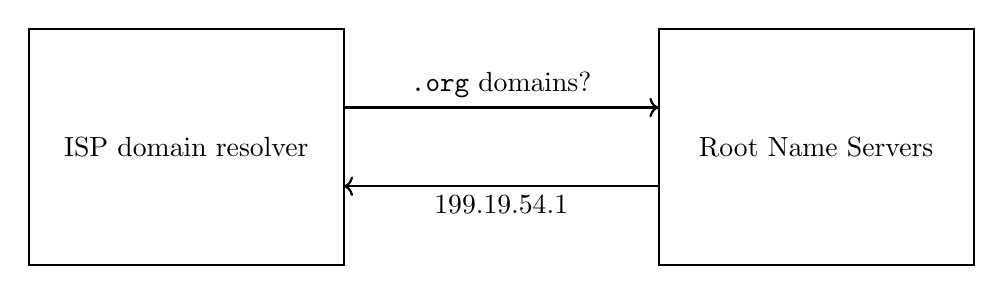
\begin{tikzpicture}
          \draw[thick] (0,0) rectangle (4,3);
          \draw[thick] (8,0) rectangle (12, 3);
          \node at (2, 1.5) {ISP domain resolver};
          \node at (10, 1.5) {Root Name Servers};
          \draw[->, thick] (4, 2)--(8,2);
          \draw[->,thick] (8,1)--(4, 1);
          \node[above] at (6, 2) {$\texttt{.org}$ domains?};
          \node[below] at (6,1) {199.19.54.1};
      \end{tikzpicture}
      \end{center}
      Then, the ISP asks the TLD name server for, say the $\texttt{wikipedia}$ domains. The TLD name server responds with the IP address of the host name server that contains the wikipedia records.
      \begin{center}
      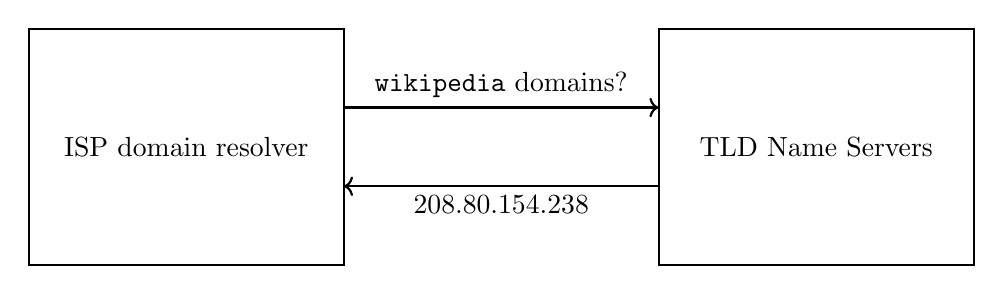
\begin{tikzpicture}
          \draw[thick] (0,0) rectangle (4,3);
          \draw[thick] (8,0) rectangle (12, 3);
          \node at (2, 1.5) {ISP domain resolver};
          \node at (10, 1.5) {TLD Name Servers};
          \draw[->, thick] (4, 2)--(8,2);
          \draw[->,thick] (8,1)--(4, 1);
          \node[above] at (6, 2) {$\texttt{wikipedia}$ domains?};
          \node[below] at (6,1) {208.80.154.238};
      \end{tikzpicture}
      \end{center}
      Finally, the ISP asks the host name server for the specific domain $\texttt{www.wikipedia.org}$. The host name server responds with an exact IP address, and now the computer can successfully connect with the computer powering that domain. 
      \begin{center}
      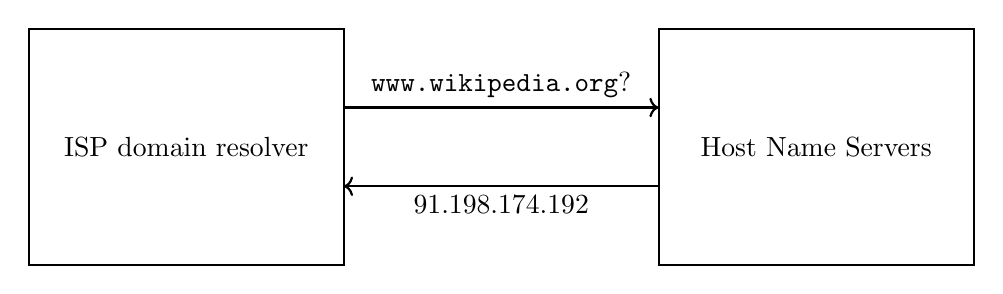
\begin{tikzpicture}
          \draw[thick] (0,0) rectangle (4,3);
          \draw[thick] (8,0) rectangle (12, 3);
          \node at (2, 1.5) {ISP domain resolver};
          \node at (10, 1.5) {Host Name Servers};
          \draw[->, thick] (4, 2)--(8,2);
          \draw[->,thick] (8,1)--(4, 1);
          \node[above] at (6, 2) {$\texttt{www.wikipedia.org}$?};
          \node[below] at (6,1) {91.198.174.192};
      \end{tikzpicture}
      \end{center}
      However, lots of information is cached, so it is rare that a \textbf{DNS lookup} has to go through all the steps. 
  \end{enumerate}

  However, the domain name system is not always secure. For example, if a cyber-criminal manages to take control of a name server or redirect requests to its own server, then it can have the server give out false IP addresses that can lead to websites filled with malware. This act is called \textbf{DNS spoofing}, or \textbf{DNS cache poisoning}. Fortunately, the recent \textbf{DNSSEC protocol} extends the original DNS protocol and specifies the best way for DNS resolvers to authenticate the information sent to them, which can prevent DNS spoofing. 

  \subsubsection{HTTP}

  Whenever a pageon the web is visited, the computer uses the \textbf{Hypertext Transfer Protocol} to download that page from another computer somewhere on the Internet. The steps of this process are as such: 
  \begin{enumerate}
      \item We access the web with a \textbf{browser application}. The user either types a \textbf{Uniform Resource Locator (URL)} in the browser or follows a link from an already opened page. 
      \item The domain names of these URLs map to IP addresses, the true location of the domain's computers. The browser uses a DNS resolver to map the domain to an IP address. 
      \item Browser sends HTTP request. Once the browser identifies the IP address of the computer hosting the requested URL (i.e. the \textbf{host computer}), it sends an \textbf{HTTP request}. An example HTTP request can be: 
      \begin{lstlisting}
      GET /index.html HTTP/1.1
      Host: www.example.com
      \end{lstlisting}
      \begin{enumerate}
          \item The word $\texttt{GET}$ is the request. There are other verbs for other actions, such as $\texttt{POST}$ for submitting form data. 
          \item The next part specifies the path ($\texttt{/index.html}$). The host computer stores the content of the entire website, so the browser needs to be specific about which page to load.
          \item The final part of the first line specifies the protocol and the version of the protocol: $\texttt{HTTP/1.1}$. 
          \item The second line specifies the domain of the requested URL. That's helpful in case a host computer stores the content for multiple websites.
      \end{enumerate}
      \item Once the host computer receives the HTTP request, it sends back a \textbf{HTTP response} with both the content and metadata about it. 
      \begin{lstlisting}
      HTTP/1.1 200 OK
      Content-Type: text/html; charset=UTF-8
      Content-Length: 208
      <!DOCTYPE html>
      <html>
          <head>
              <title>Example Domain</title>
          </head>
          <body>
              <h1>Example Domain</h1>
              <p>This domain is to be used for illustrative examples in documents.</p>
          </body>
      </html>
      \end{lstlisting}
      \begin{enumerate}
          \item The $\texttt{HTTP/1.1}$ is the protocol and version. The next number is the \textbf{HTTP status code}. In this case, a $\texttt{200}$ represents a successful retrieval of the document, "OK." Another code is the $\texttt{404}$ code, which represents "file not found."
          \item The 2nd and 3rd lines are the \textbf{headers}, which provides additional details. The content-type tells the browser what type of document is being sent back. $\texttt{text/html}$ represent HTML text files; $\texttt{image/png}$ represent images; $\texttt{video/mpeg}$ are videos; $\texttt{application/javascript}$ are scripts; and so on. The content length gives the length of the document in bytes. 
          \item The rest of the HTTP response writes our the actual document requested. 
      \end{enumerate}
      \item The browser renders the response, and you see the regular webpage. 
  \end{enumerate}

  Note that HTTP is a protocol that is built on top of the TCP/IP protocols. That is, each HTTP request/response is inside an IP packet (or more often, in multiple packets). There are many other protocols built on top of TCP/IP, like protocols for sending email (SMTP, POP, IMAP) and uploading files (FTP). 

  Note that the protocols powering the Internet and the Web were designed for scalability. Any computing device can send data around the Internet if it follows the protocols, and routing is dynamic, so new routers can join a network at any time and help to move data packets around the internet.

  \begin{definition}
  A \textbf{scalable system} is one that can continue functioning well even as it experiences higher usage. 
  \end{definition}

  However, there are limitations to the scalability of the internet. For example, 
  \begin{enumerate}
      \item Network connections have limited bandwidth, so huge amounts of data could easily overwhelm low bandwidth connections, leading to delays or dropped packets. 
      \item Routers have limited throughput (the amount of data they can forward per second). A modern consumer router has a throughput around 1 Gbps while much more expensive enterprise routers can forward up to 10 Gbps. 
      \item Wireless routers often have a limitation in the number of devices that can be connected to them, typically up to 250 devices. If everyone tried to use a shared WiFi network at the same time (like in a university or library), they might find themselves simply unable to join.
  \end{enumerate}

  \begin{definition}
  Engineering teams can prepare for spikes in usage by doing \textbf{load testing}: simulating high amounts of traffic in a short period of time to stress test the system. Load testing can uncover bottlenecks or hard-coded limits in the system. 
  \end{definition}

  \subsection{The Internet Protocol Suite}
  There are many protocols that power the Internet. Each protocol operates at a different layer, building functionality on top of the layer below it. We can visualize it in the following diagram. 
  \begin{center}
  \begin{tabular}{l|l}
      Application Layer & HTTP, TLS, DNS\\
      \hline
      Transport Layer & TCP, UDP \\
      \hline
      Network Layer & IP (v4, v6) \\
      \hline
      Link Layer & Ethernet, Wireless LAN
  \end{tabular}
  \end{center}
  \begin{enumerate}
      \item At the link layer, 2 computing devices need a physical mechanism to send digital data to each other. They send electromagnetic signals either over a wired or wireless connection and interpret the signal as bits. This type of physical connection affects the bit rate and bandwidth. 
      \begin{center}
      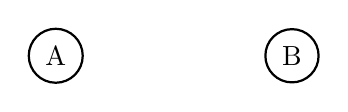
\begin{tikzpicture}[-,>=stealth',shorten >=1pt,auto,node distance=3cm, thick,main node/.style={circle,draw}, every loop/.style={}]
      \node[main node] (A) {A};
      \node[main node] (B) [right of=A] {B};
      \end{tikzpicture}
      \end{center}
      \item Once a network is bigger than two computers, we need addressing protocols to uniquely identify who is sending data and who should receive the data. Every node on the Internet is identified with an IP address.
      \begin{center}
      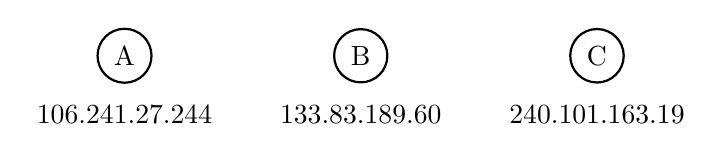
\begin{tikzpicture}[-,>=stealth',shorten >=1pt,auto,node distance=3cm, thick,main node/.style={circle,draw}, every loop/.style={}]
      \node[main node] (A) {A};
      \node[main node] (B) [right of=A] {B};
      \node[main node] (C) [right of=B] {C};
      \node[below] at (0,-0.5) {106.241.27.244};
      \node[below] at (3,-0.5) {133.83.189.60};
      \node[below] at (6,-0.5) {240.101.163.19};
      \end{tikzpicture}
      \end{center}
      \item The route between any two computers on the Internet isn't just a straight path from A to B. The data must pass from router to router until it finally reaches its destination, a strategy that comes from the Internet routing protocol.
      \begin{center}
      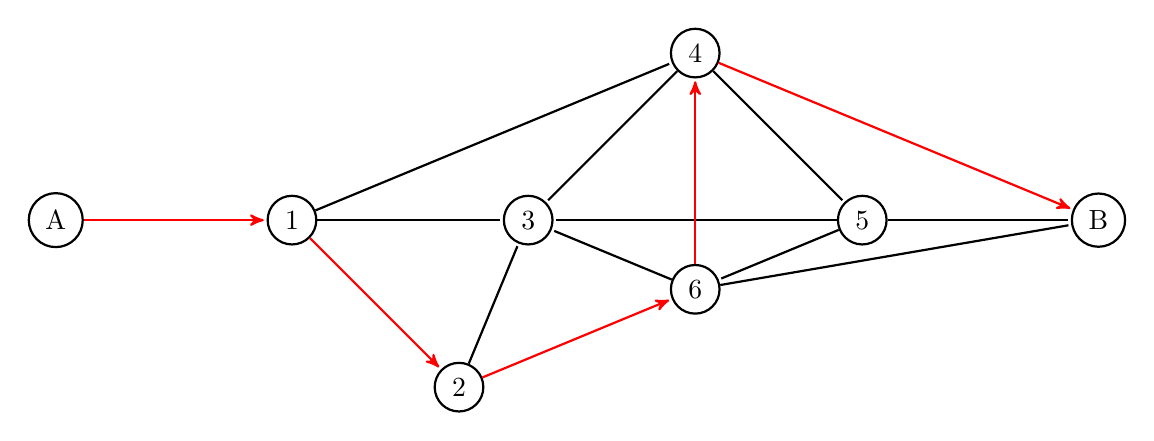
\begin{tikzpicture}[-,>=stealth',shorten >=1pt,auto,node distance=3cm, thick,main node/.style={circle,draw}, every loop/.style={}]
      \node[main node] (A) {A};
      \node[main node] (1) [right of=A] {1};
      \node[main node] (2) [below right of=1] {2};
      \node[main node] (3) [right of=1] {3};
      \node[main node] (4) [above right of=3] {4};
      \node[main node] (5) [below right of=4] {5};
      \node[main node] (B) [right of=5] {B};
      \node[main node] (6) [below of=4] {6};
      \path[every node/.style={font=\sffamily\small}]
      (A) edge[red, ->] node {} (1)
      (1) edge node {} (3)
      (1) edge[red, ->] node {} (2)
      (1) edge node {} (4)
      (2) edge node {} (3)
      (4) edge node {} (3)
      (5) edge node {} (3)
      (2) edge[red, ->] node {} (6)
      (5) edge node {} (B)
      (5) edge node {} (6)
      (6) edge node {} (3)
      (6) edge[red, ->] node {} (4)
      (4) edge node {} (5)
      (4) edge[red,->] node {} (B)
      (6) edge node {} (B);
      \end{tikzpicture}
      \end{center}
      \item Data needs to be broken up into small packets, which are then reassembled at the destination. The Transmission Control Protocol (TCP) is used to ensure reliable transport of those packets, with sequencing, acknowledgement, and retries. A faster but less reliable transport protocol is the User Datagram Protocol (UDP).
      \begin{center}
      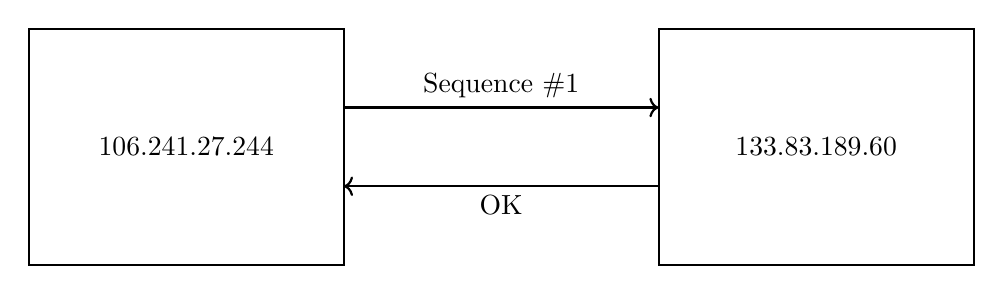
\begin{tikzpicture}
          \draw[thick] (0,0) rectangle (4,3);
          \draw[thick] (8,0) rectangle (12, 3);
          \node at (2, 1.5) {106.241.27.244};
          \node at (10, 1.5) {133.83.189.60};
          \draw[->, thick] (4, 2)--(8,2);
          \draw[->,thick] (8,1)--(4, 1);
          \node[above] at (6, 2) {Sequence \#1};
          \node[below] at (6,1) {OK};
      \end{tikzpicture}
      \end{center}
  \end{enumerate}
  The Transport Layer Security (TLS) protocol uses algorithms to encrypt the data (cryptography). \textit{Certificate authorities} help users trust the encryption. 

  \begin{example}
  When loading a webpage from a domain your browser has never visited before, your browser may need to make a DNS request, which is represented by the following stack of protocols when the request is sent through the internet. 
  \begin{center}
  \begin{tabular}{l|l}
      Application Layer & DNS\\
      Transport Layer & UDP \\
      Network Layer & IP \\
      Link Layer & Wireless LAN
  \end{tabular}
  \end{center}
  Then, your browser will make an HTTP request to fetch the webpage. This prototol stack is used when an HTTP request is sent:
  \begin{center}
  \begin{tabular}{l|l}
      Application Layer & HTTP\\
      Transport Layer & TCP \\
      Network Layer & IP \\
      Link Layer & Wireless LAN
  \end{tabular}
  \end{center}
  If the webpage is served over HTTPS, then the stack includes multiple protocols at the application layer (both HTTP and TLS): 
  \begin{center}
  \begin{tabular}{l|l}
      Application Layer & HTTP, TLS\\
      Transport Layer & TCP \\
      Network Layer & IP \\
      Link Layer & Wireless LAN
  \end{tabular}
  \end{center}
  \end{example}

  In a network, we must also make sure that the computers follow the \textit{same} protocol, i.e. there is \textit{standardization} within the network. Fortunately, the protocols of the Internet are \textbf{open} (not owned by any particular company and not limited to a particular company's products). For every protocol that is both standardized and open, there is a publicly viewable document describing the protocol, often called the \textbf{specification}. These specifications are maintained by the \textbf{Internet Engineering Task Force (IEFT)}. Some of them are: 
  \begin{enumerate}
      \item the HTTP specification
      \item the TCP specification
  \end{enumerate}
  The languages of the web are also open standards with online specifications. They include the
  \begin{enumerate}
      \item HTML living standard
      \item many specifications for CSS
      \item ECMAScript standard for JavaScript. 
  \end{enumerate}

  \subsubsection{Checking Network Processes}
  To check all open network connections (by process) and their usage of network bandwidth, use the $\texttt{nettop}$ keyword on the command line. This can be used to find out which processes are taking up all of your local network bandwidth. 
  \begin{lstlisting}
  >>>nettop 
                              interface       state    bytes_in  bytes_out
  systemstats.64                                            0 B        0 B
  udp4 *:*<->*:*

  config.66                                                 0 B        0 B
  udp4 *:*<->*:*

  remoted.71                                            489 KiB    680 KiB 
  tcp6 IPv6\%en3.49160<->*.*        en3      Listen      
  tcp6 IPv6\%en3.49160<->IPv6       en3 Established     494 KiB    687 KiB

  apsd.97                                                18 KiB     21 KiB
  tcp4 IPv4:52737<->IPv4:5223       en0 Established      18 KiB     21 KiB

  timed.99                                                144 B      144 B

  usbmuxd.100                                           104 KiB     75 KiB
  tcp4 IPv4:52695<->IPv4:54848      en0 Established     104 KiB     75 KiB
   
  bluetooth.119                                             0 B        0 B
  udp4 *:*<->*:*

  AirPlayXPCHelpe.123                                       0 B        0 B
  udp4 *:*<->*:*
  udp4 *:*<->*:*

  loginwindow.131                                           0 B        0 B
  udp4 *:*<->*:*

  mDNSResponder.164                                    6996 KiB   2606 KiB
  udp6 *.5353<->*.*                 lo0                1717 KiB    790 KiB
  udp4 *.5353<->*:*                 en0                5235 KiB   1808 KiB

  symptomsd.189                                             0 B        0 B
  udp4 *:*<->*:*

  findmydeviced.190                                      1349 B     3061 B
  tcp6 IPv6\%en3.49161<->IPv6.49248 en3 Established      1349 B     3061 B

  airportd.198                                              0 B        0 B
  udp4 *:*<->*:*
  udp4 *:*<->*:*
  udp4 *:*<->*:*
  udp6 *:*<->*:*
  udp4 *:*<->*:*

  corekdld.203                                            293 B     31 KiB
  tcp6 IPv6\%en3.49163<->IPv6.49256 en3 Established       293 B     31 KiB

  bosUpdateProxy.204                                      406 B     2903 B
  tcp6 IPv6\%en3.51336<->IPv6.49260 en3 Established       406 B     2903 B

  #Only the processes will be shown from now on. 

  SubmitDiagInfo.205                                    65 KiB        9210 B
  mobileactivatio.206                                   9238 B        11 KiB
  locationd.270                                            0 B           0 B
  biometrickitd.290                                    509 KiB        95 KiB
  accountsd.338                                         5518 B        1247 B
  trustd.342                                            4363 B         610 B
  Simplenote.355                                        6316 B        6661 B
  rapportd.356                                          10 KiB        4965 B
  ControlCenter.359                                        0 B           0 B
  Finer.361                                                0 B           0 B
  identityservice.369                                   4600 B        2961 B
  itunescloudd.374                                      30 KiB        2533 B
  com.apple.geod.392                                    3512 B        1353 B
  WirelessRadioMa.414                                      0 B           0 B
  sharingd.417                                             0 B           0 B
  nsurlsessiond.420                                      6 KiB        9246 B
  CalendarAgent.424                                     95 KiB        39 KiB
  wifivelocityd.426                                        0 B           0 B
  NewsToday2.437                                       392 KiB        27 KiB
  AMPDeviceDiscov.441                                   2602 B        3725 B
  assistantd.453                                        22 KiB        8764 B
  ScreenTimeWidge.463                                   8029 B         936 B
  WeatherWidget.464                                     7471 B        1168 B
  corespeechd.471                                       7226 B        25 MiB
  com.apple.Safar.530                                   11 KiB        2478 B
  AdobeDesktop S.616                                       0 B           0 B
  node.640                                                 0 B           0 B
  comapple.WebKi.1274                                   17 MiB       627 KiB
  com.appleSafar.1335                                   9956 B        2303 B
  PowerChime.1353                                       2853 B        19 KiB
  adprivacyd.1388                                       24 KiB        5253 B
  lskdd.1768                                            1805 B        5851 B
  PerfPowerServic.15327                                    0 B           0 B
  netbiosd.19203                                       277 KiB       142 KiB
  bluetoothaudiod.19268                                    0 B           0 B
  Notify.20116                                             0 B           0 B
  \end{lstlisting}
  Note that pressing $\texttt{q}$ quits nettop; pressing $\texttt{p}$ renders the traffic numbers as bytes or in human-readable formats; pressing $\texttt{c}$ collapses the display, showing only the network apps (no sockets); pressing $\texttt{e}$ expands the display to show sockets. 

  Under each process (network application) there is a list of \textbf{sockets}, which are endpoints in a two-way communication between two programs on a network; for example, between a web server and your web browser. Looking at the columns, 
  \begin{enumerate}
      \item The leftmost column contains the list of all the names of the processes and sockets, followed by a dot and their process ID (PID); so in the form
      \[\texttt{NetworkApp.PID}\]
      For example, $\texttt{locationd.270}$ would be the process locationd with a PID of 270. 
      \item A \textbf{network interface} is the point of interconnection between a computer and a private/public network. The \textit{network interface card} connects your computer to a local data network or the internet. The card translates computer data into compatible electrical signals it sends through the network. 
      \begin{enumerate}
          \item $\texttt{lo0}$ is loopback interface. A \textbf{loopback} is the routing of electronic signals, digital data streams, or flows of items back to their source without intentional processing or modification. It is primarily a means of testing the transmission tests. 
          \item $\texttt{en0}$ is Wifi (was ethernet at one point)
          \item $\texttt{fw0}$ is the FireWire network interface 
          \item $\texttt{utun1}$
          \item $\texttt{stf0}$ is an IPv6 to IPv4 tunnel interface to support the transition from IPv4 to IPv6 standard. 
          \item $\texttt{gif0}$ is a more generic tunneling interface. 
          \item $\texttt{awdl0}$ is Apple Wireless Direct Link
      \end{enumerate}
      \item The \textbf{state} refers to the state of the connection between sockets. 
      \begin{enumerate}
          \item The state of a server waiting for a connection on a port is $\texttt{Listen}$
          \item The state of a connection recently closed is $\texttt{TimeWait}$ 
          \item $\texttt{Established}$ means that the connection is active
          \item $\texttt{SynSent}$ occurs when a client initiates the connection to a server by sending the SYN packet (a part of the 3-way handshake in TCP) and awaits the ACK packet. 
      \end{enumerate}
      \item The $\texttt{bytes\_in}$ and $\texttt{bytes\_out}$ shows how much traffic has come in and gone out for that socket (or for the entire process).
  \end{enumerate}

  The format of each socket is
  \[\texttt{TransportProtocolVersion localhostIPaddress:port<->remoteIPaddress:port}\]
  Notice that all of the sockets use the standardized UDP or TCP protocol (with the corresponding IP address Version: IPv4 or IPv6). 
  \begin{enumerate}
      \item $\texttt{udp4, udp6}$ - the connection is one-way since there are no SYN and ACK bits being sent to confirm the connection. 
      \item $\texttt{tcp4, tcp6}$ - the connection guarantees that both ends are aware of one other, so datagrams can be sent back and forth until the FIN bit is sent and acknowledged. 
  \end{enumerate}
  A transport protocol (say, tcp) that use IPv4 is in the form
  \[\texttt{tcp4 192.168.0.88:52737<->17.57.145.138:5223}\]
  while one that uses IPv6 is in the form 
  \[\texttt{tcp6 fe80::aede:48ff:fe00:1122\%en3.4915<->fe80::aede:48ff:fe33:445\%en3.5960}\]
  Some sockets may have asterisks rather than actual IP addresses in them. 
  \begin{lstlisting}
  airportd.198                                              0 B        0 B
  udp4 *:*<->*:*
  udp4 *:*<->*:*
  udp6 *:*<->*:*
  \end{lstlisting}
  An asterisk means that these sockets are open. The operating system creates these open sockets as placeholders of sorts, so that it can respond faster to incoming data (since incoming data will trigger the creation of a socket, which causes delay). 

  \begin{definition}
  In addition to the IP address, the \textbf{port number} is the part of the addressing information used to determine what protocol incoming traffic should be directed to. That is, port number identifies a specific process to which an Internet or other network message is to be forwarded when it arrives at a server. They are represented by 16-bit numbers, meaning that port numbers can have values up to $2^{16} = 65,536$. However,
  \begin{enumerate}
      \item 0-1023 are restricted port numbers and are used by well-known protocol services. Some of them include:
      \begin{enumerate}
          \item 80 for HTTP
          \item 123 for NTP
          \item 67, 68 for DHCP traffic
          \item 443 for HTTPS (almost all ports in the browser socket will be 443). 
          \item 137, 138 for netbios. NetBIOS is a protocol used for File and Print Sharing under all current versions of Windows. 
      \end{enumerate}
      \item 1024-49,151 are registered port numbers; they can be registered to specific protocols by software corporations.
      \item 49,152-65,536 are used as dynamic/private ports and can be used by anybody. 
  \end{enumerate}
  \end{definition}

  The differences between the IP address and port number are: 
  \begin{enumerate}
      \item The IP address is used to identify a host in the network, while a port number is used to identify a process/service on your system. 
      \item IP address is the address of the layer-3 Internet protocol suite, while the port number is the address of the layer-4 protocols. 
      \item IP address is provided by admin of system or network administrator, while the port number is provided by the kernel of the operating system. 
  \end{enumerate}


  \subsection{Online Data Security}

  \begin{definition}
  \textbf{Personally identifiable information (PII)} refers to data that can directly or indirectly identify individuals. Some of the most common PIIs are: 
  \begin{enumerate}
      \item Name 
      \item Social Security Number
      \item Biometric Data (DNA, fingerprints, etc.)
  \end{enumerate}
  Another weaker form of PII are \textbf{linkable PII}, which refers to data that can be combined from separate sources to identify individuals. 
  \end{definition}

  It is hard to classify certain data as PII or not since the capabilities and the creative use of them is changing. An instance of when attackers steal PII from companies is known as a \textbf{data breach}. You can check whether you are a victim of a data breach with services like $\texttt{haveibeenpwned.com}$. 

  The web is not private by default; websites often use \textbf{cookies} to track user action on their site and even across other sites (to improve their services).

  \begin{definition}
  An \textbf{HTTP cookie} is a small amount of text that helps a website track information about a user across multiple pages of the website and personalize the user's experience on the website. 
  \end{definition}

  If you've ever logged into a website, a cookies kept you logged in across multiple pages. A cookie is set in the following steps: 
  \begin{enumerate}
      \item When a user navigates to a website for the first time (in a particular browser), the browser sends an HTTP request to the server that hosts the website. 
      \begin{lstlisting}
      GET /index.html HTTP/1.1
      Host: www.shoopshop.com
      \end{lstlisting}
      \item The server sends back an HTTP response and includes a $\texttt{Set-cookie}$ header in that response. 
      \begin{lstlisting}
      HTTP/1.0 200 OK
      Content-type: text/html
      Set-Cookie: sessionId=abc123; Expires=Wed, 09 Jun 2021 10:18:14 GMT
      ...
      \end{lstlisting}
      The cookie contains a name ($\texttt{sessionId}$) and a value ($\texttt{abc123}$), plus an expiration date for the browser to clear this cookie from its memory. If it wants to set multiple cookies, it adds more $\texttt{Set-cookie}$ headers to the response. 
      \item The browser saves the cookie information, storing it on the user's hard drive. That way, the data will persist even after restarting the browser or computer, which is why this type of cookie is called a \textbf{persistent cookie}. There are also \textbf{session cookies} which have no expiration date and are always deleted when the browser is shut down. 
      \item When the user navigates to a different page on the website, the browser sends along the stored cookies with each HTTP request. 
      \begin{lstlisting}
      GET /shop.html HTTP/1.1
      Cookie: sessionId=abc123
      \end{lstlisting}
      \item When the server receives the HTTP request, it inspects the cookies and sees that this request is coming from a user with a known $\texttt{sessionId}$. It can then look up that session ID in its database and use any information about the session to personalize the response. 
  \end{enumerate}

  Cookies can have many uses, such as: 
  \begin{enumerate}
      \item A search engine can use them to remember how many results a user prefers seeing per page.
      \item A news site can use them to recommend headlines that are similar to the articles you've already read. 
      \item All sorts of websites can use cookies to track analytics, like how long you spent on a page and which buttons you clicked.
      \item Any website with a log-in uses a cookie to keep you logged in on every page of the site. When you log out of that site, it clears the cookie and doesn't set it again until you login again.
  \end{enumerate}
  It is clear that you should never share your cookies. 

  \begin{definition}
  Each cookie stored by a browser is associated with a domain and path. When you visit a website and its server sends back an HTTP response with a cookie, the browser associates that cookie with the domain of the server. That's called a \textbf{first-party cookie}. 

  However, a website can also include resources from other domains, like an image, iframe, or script. When the browser requests those resources, their servers can also send back cookies, which will now be associated with their domain. These are called \textbf{third-party cookies}.
  \end{definition}

  Imagine a user that visits a food blog with a recipe for gluten-free cookies. That blog includes a Facebook ad with a cookie. The user then visits $\texttt{facebook.com}$ and notices a sudden uptick in ads about gluten-free products, which resulted from the cookies in the Facebook ad in the blog. Third-party cookies more often serve the purpose of collecting information for advertising and infringe more on the privacy of web users. 

  \subsubsection{Search and Browsing History}
  \begin{definition}
  A \textbf{search engine} is a service that builds an index of the World Wide Web and gives users a way to search that index. 
  \end{definition}

  It is important to know that in order to improve their services (like spelling correction) all search engines collect data on search queries (i.e. what was searched). A search query itself isn't private information, but some search engines can log much more than the query: 
  \begin{center}
  \begin{tabular}{l|l|l|l|l}
      Search query & Date & Time & IP address & User agent \\
      \hline 
      "jet ski" & 03/11/20 & 11:14 & 49.121.111.73 & Mozilla/5.0 (Windows NT 5.1) \\
      "home depot" & 03/11/20 & 16:00 & 49.121.111.73 & Mozilla/5.0 (Windows NT 5.1) \\
      "cheap pizza" & 03/12/20 & 21:07 & 49.121.111.73 & Mozilla/5.0 (Windows NT 5.1) \\
      "Windsor" & 03/13/20 & 14:32 & 49.121.111.73 & Mozilla/5.0 (Windows NT 5.1) 
  \end{tabular}
  \end{center}
  A combination of these queries over a period of time can definitely be PII, and additionally, the search history can include a cookie or even a user ID if you were logged into the search engine website when you issued the query. Third party cookies can allow a website to track a user's browsing history across other websites, as long as each site loads the cookie from the same domain. 

  Many browsers also provide an \textit{incognito browsing mode}, which will not store browsing history at all. Once you close the window, it will also forget any cookies generated in that session. There are certain search engines, such as DuckDuckGo, that collect only search queries and do not collect any PII.

  Note that since all requests (packets of data) are forward through the router, anyone with access to the router can monitor the destinations of HTTP requests. An Internet Service Provider (ISP) administers the first routers that a packet travels through (excluding the home/office/school) router, so the ISP can see every HTTP request that's sent through those routers. Users can use HTTPS-secured websites to hide the contents of their requests, but HTTPS will still reveal the domain names. ISPs can use that information to find customers that are engaged in illegal activities, such as downloading pirated movies. Government organization such as the National Security Agency (NSA) have reportedly installed backdoor surveillance monitoring programs on routers before they were exported to foreign customers. 

  \subsubsection{VPNs and Tor}
  \begin{definition}
  When using a \textbf{Virtual Private Network (VPN)}, the computer sends a packet of encrypted data with a destination of the VPN server to the ISP. The VPN server decrypts the data, finds out where the user actually wants to send the packet, and then forwards the packet to that destination. 
  \begin{center}
  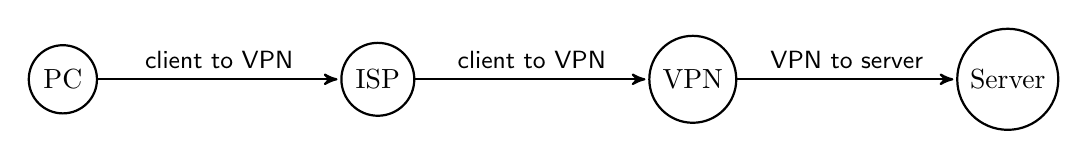
\begin{tikzpicture}[->,>=stealth',shorten >=1pt,auto,node distance=4cm, thick,main node/.style={circle,draw}, every loop/.style={}]
      \node[main node] (PC) {PC};
      \node[main node] (ISP) [right of=PC] {ISP};
      \node[main node] (VPN) [right of=ISP] {VPN};
      \node[main node] (Server) [right of=VPN] {Server};
      \path[every node/.style={font=\sffamily\small}]
      (PC) edge node {client to VPN} (ISP)
      (ISP) edge node {client to VPN} (VPN)
      (VPN) edge node {VPN to server} (Server);
  \end{tikzpicture}
  \end{center}
  The VPN server knows the user's browsing history, but the ISP does not. Plus, other routers after the VPN will only see that the packet came from the VPN IP address, not from the user's IP address. A VPN subscription is often expensive, however, and the additional stop along the way can result in a slower browsing experience. 
  \end{definition}

  Another option is \textbf{Tor}, an open source program for anonymizing Internet traffic.  When using Tor, the computer sends an encrypted packet through a large number of volunteer relays. The data is packaged such that each relay only knows where it came from and where it's going, and no relay knows both the sender IP address and the destination IP address. 
   
  Tor can provide truly anonymous browsing, but it also severely slows down the browsing experience, since it has to hop through volunteer relays that can be located anywhere on the Internet. 

  \begin{definition}
  A \textbf{proxy server} is a server application or appliance that acts as an intermediary for requests from clients seeking resources from servers that provide those resources. A proxy server thus functions on behalf of the client when requesting service, potentially masking the true origin of the request to the resource server. 

  Instead of connecting directly to a server that can fulfill a requested resource, such as a file or web page, the client directs the request to the proxy server, which evaluates the request and performs the required network transactions. This serves as a method to simplify or control the complexity of the request, or provide additional benefits such as load balancing, privacy, or security. Proxies were devised to add structure and encapsulation to distributed systems. Some types of proxies are: 
  \begin{enumerate}
      \item A \textbf{gateway} or a \textbf{tunneling proxy} is a proxy server that passes unmodified requests and responses. 
      \item An \textbf{open proxy} is a forwarding proxy server that is accessible by any Internet user. Hundreds of thousands of open proxies are operated on the internet. 
      \begin{enumerate}
          \item \textbf{Anonymous proxies} reveals its identity as a proxy server, but does not disclose the originating IP address of the client. 
          \item \textbf{Transparent proxies} also identifies itself as a proxy server, but the originating IP address can be retrieved. The main benefit of using this type of server is its ability to cache a website for faster retrieval. 
      \end{enumerate}
      \item A \textbf{reverse proxy} is a proxy server that appears to clients to be an ordinary server. Reverse proxies forward requests to one or more ordinary servers that handle the request. The response from the proxy server is returned as if it came directly from the original server, leaving the client with no knowledge of the original server. Reverse proxies aer installed in the neighborhood of one or more web servers, and all traffic coming from the Internet goes through the proxy server. The use of \textit{reverse} originates in its counterpart \textit{forward proxy} since the reverse proxy sits closer to the web server and serves only a restricted set of websites. 
      \begin{enumerate}
          \item Encryption/SSL acceleration: When secure websites are created, the \textit{Secure Sockets Layer (SSL)} encryption is often not done by the web server itself, but by a reverse proxy that is equipped with SSL acceleration hardware. 
          \item Load balancing: the reverse proxy can distribute the load to several web servers, each web server serving its own application area. 
          \item Serve/cache static content: A reverse proxy can offload the web servers by caching static content like pictures and other static graphical content.
          \item Compression: the proxy server can optimize and compress the content to speed up the load time.
          \item Security: the proxy server is an additional layer of defense and can protect against some OS and Web Server specific attacks. However, it does not provide any protection from attacks against the web application or service itself, which is generally considered the larger threat.
      \end{enumerate}
  \end{enumerate}
  \end{definition}

  \subsubsection{Geolocation}

  \begin{definition}
  The \textbf{geolocation} of a device is an approximate latitude and longitude describing its geographic location. 
  \end{definition}

  \begin{definition}
  The most popular method in which geolocation is determined is through \textbf{trilateration}, which is a geometric process of of determining absolute or relative locations of points by measurements of distances, using the geometry of circles, spheres ,or triangles. For example, given three points $A, B, C \in \mathbb{R}^2$, a unique point with certain distances from $A, B, C$ can be determined. 
  \begin{center}
  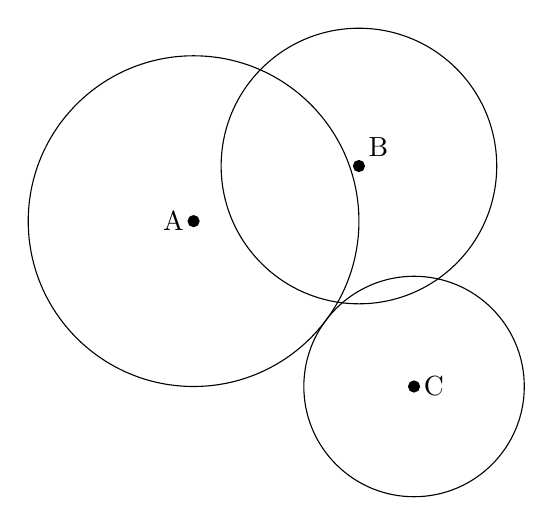
\begin{tikzpicture}[scale=0.7]
      \draw (-1,0) circle (3);
      \draw (2,1) circle (2.5);
      \draw (3,-3) circle (2);
      \draw[fill] (-1,0) circle (0.1); 
      \draw[fill] (2,1) circle (0.1); 
      \draw[fill] (3,-3) circle (0.1); 
      \node[left] at (-1,0) {A};
      \node[above right] at (2,1) {B};
      \node[right] at (3,-3) {C};
  \end{tikzpicture}
  \end{center}
  Other methods of trilateration exist. 
  \end{definition}

  One way to determine geolocations is through the \textbf{Global Position System (GPS)}, a project started by the US government in the 1970s controlled by approximately 30 GPS satellites orbiting the Earth. \textbf{GPS receivers} are tiny sensors with antennas that receive radio signals from the GPS satellites orbiting in the sky above. If a sensor can receive signals from at least 4 satellites, the receiver can calculate its position using trilateraion. Since they depend on radio signals from satellites, GPS is most accurate in an outdoor environment with a clear view of the sky. 

  On the other hand, \textbf{WiFi positioning} is a strategy that works well in dense, urban areas filled with WiFi networks. First, a device with a WiFi antenna scans for WiFi access points and measures the signal strength to each network. (Note that signal strength is always negative, so the number closest to 0 is strongest)
  \begin{center}
  \begin{tabular}{l|l|l}
      BSSID & MAC address & Signal strength (RSSI) \\
      \hline
      NETGEAR09 & A3:F3:5D:2A:A3:1B & -59 \\
      NETGEAR09-5G & A3:F3:5D:2A:A3:1B & -72 \\
      Sonic-b346 & 53:19:DA:E0:57:3A & -79 \\
      Emdutos & E3:84:14:BC:BC:FF & -84 \\
      Baskind Bunch & 52:8D:5E:29:E7:5A & -85 \\
      Sonic-9472-5G & 4C:4C:DB:91:1A:1A & -88 \\
      xfinitywifi & F8:59:F4:FC:C5:F1	& -93
  \end{tabular}
  \end{center}
  Then, the device determines the location of each access point by looking it up in a WiFi location database or in their own (smaller) cache of locations. It then estimates its own location based on the found locations and their signal strength using trilateration. 

  A more accurate technique is \textbf{fingerprinting}, but only possible if a fingerprint map has been made ahead of time. To make the map, a portable device computes the fingerprint for many reference points within a particular area. Each fingerprint is the list of nearby networks and their signal strength, like the table above, plus a pair of geographic coordinates. When a mobile device enters the area and needs to know its location, it can send its fingerprint to the machine with the radio map, and the machine uses an algorithm to compute the closest fingerprint and estimate the coordinates accordingly. This is basically just using WiFi positioning ahead of time. 

  If a cell phone is unable to use GPS to report its location, it can instead use \textbf{cell tower trilateration}. Cell towers are what makes cellular networks possible. Each cell tower includes three sets of directional antenna arrays in a triangular shape, and using trilateration, multiple cell towers can be used to determine the geolocation of a mobile device. 

  The least accurate of all methods is \textbf{IP-based geolocation}. IP geolocation databases contain millions of rows mapping IP addresses to locations. Companies create those databases based on a variety of sources such as regional IP address registries, user-submitted locations on websites, data from ISPs, and estimates based on network routes. They usually get the country and state correct, but often there are deviations in any more specific location data. Furthermore, if a user is accessinfg the Internet through a VPN, their true IP will be hidden and the VPN's IP could be geolocated in an entirely different continent. 

  Note that when a user visits a website, their browser sends an HTTP request to the web server. The HTTP request is wrapped in an IP packet, so it always includes the sender's IP address. Therefore, the web server can always use an IP geolocation service to turn the user's IP address into an approximate location, which can give better demographics for the company. 

  \subsection{Cyber Attacks}

  A \textbf{phishing attack} is an attempt to trick a user into divulging their private information. Some signs of a phishing attack are: 
  \begin{enumerate}
      \item suspicious email addresses. However, a legitimate email address is not a guarantee that an email is 100\% safe. Attackers mught have figured out a way to spoof the legitimate email address or hacked their way into control over the actual email. 
      \item Suspicous URL. Attackers may
      \begin{enumerate}
          \item misspell the original URL ($\texttt{goggle.com}$)
          \item use similar looking characters from other alphabets (the $\texttt{e}$ and $\texttt{a}$) in $\texttt{wikipedia.org}$ are actually different characters in those two domains)
          \item subdomains that look like the domain name. ($\texttt{paypal.accounts.com}$ vs $\texttt{accounts.paypal.com}$)
          \item have a different top level domain (TLD) ($\texttt{paypal.io}$ vs $\texttt{paypal.com}$). Popular companies try to buy their domain with the most common TLDs, such as $\texttt{.net, .com, .org}$, but there are hundreds of TLDs out there. 
          \item Have a hyperlinked text directed to a different URL. 
      \end{enumerate} 
      \item Phishing websites sometimes may not use HTTPS. Any website that is asking you for sensitive information should be using HTTPS to encrypt the data sent over the Internet.
  \end{enumerate}

  \begin{definition}
  An \textbf{access point} acts as a translator between wireless and wired signals. Access points connect to the Internet via a wired connection but share it wirelessly with many devices like your computer. Most routers include access points since they are responsible for transporting packets, not for providing wireless Internet access. Most of them have an Ethernet cable in the back that connects it to the Internet and antennae that broadcase and receive wireless signals. 
  \end{definition}

  However, another form of cyberattacking is through \textbf{rogue access points}, which an access point installed on a network without the network owner's permission. If an attacker owns the access point, they can intercept the data (PII) flowing through the network. There are two ways rogue access points can intercept PII: 
  \begin{enumerate}
      \item \textit{Passive interception}. A rogue access point can read your data but cannot manipulate it. If you connect to a network with a rogue access point and enter your password on a site over HTTP, the rogue access point can read your password. They also have access to your Internet footprint. 
      \item \textit{Active interception}. In active interception, a rogue access point can also manipulate your data. They can read the incoming user data, modify the data however they want, and send the modified user data to the destination endpoint. For example, if a user visits a banking website and tries to deposit money into an account, a rogue access point can redirect the deposit to an attacker’s account. 
  \end{enumerate}

  We can also protect ourselves by using VPNs (virtual private networks) or HTTPS. VPNs and HTTPS both send an encrypted form of our data across the network. Even if rogue access points intercept it, they won’t be able to unscramble it. 

  \begin{definition}
  \textbf{Malware} is malicious software that is unknowningly installed onto a computer and often tries to steal personal data or make money off the user. 
  \begin{enumerate}
      \item A \textbf{trojan horse} is a harmful program that masquerades as a legitimate program. 
      \item A \textbf{virus} is self-replicating: it contains code that copies itself into other files on the system. Viruses may hide in the code of a legitimate program. 
      \item A \textbf{worm} is also self-replicating, but copies itself into entirely different computers within the network. It can travel along networked protocols such as email, file sharing, or instant messaging. 
  \end{enumerate}
  The effects of malware are: 
  \begin{enumerate}
      \item \textbf{Spyware} steals data and sends it back to the malware creators. A common form of spyware are keyloggers, programs that monitor everything a user types including passwords. 
      \item \textbf{Adware} pops up advertisements to users.
      \item \textbf{Ransomware} holds a computer hostage y encrypting user data or blocking access to applications, and it demands the user pay a ransom to the anonymous malware creators. 
      \item \textbf{Cryptomining malware} utilizes a computer's resources to mine for cryptocurrency. That allows the creators to earn cryptocurrency without needing to spend money on powering their own computers.
  \end{enumerate}
  \end{definition}

  Some protection mechanisms against malware include: 
  \begin{enumerate}
      \item A security patch is an update to the code of an application or the entire operating system, and often fixes a bug that's been exploited by malware. 
      \item A \textbf{firewall} is a system that monitors incoming and outgoing network traffic to a computer or internal network, and determines what traffic to allow. Firewalls can do automated detection of suspicious traffic and can also be configured manually. 
      \item Antivirus software protects an individual computer by constantly scanning files and identifying malware. Once an antivirus program finds a piece of malware, it can guide the user through deleting or repairing the file to be safe again. 
  \end{enumerate}

  \subsubsection{Secure Internet Protocols}
  We assume that the reader is familiar with basic encryption techniques, including public-key encryption. 

  \begin{definition}
  A \textbf{symmetric encryption} is any technique where the same key is used to both encrypt and decrypt the data (e.g. the Caesar Cipher, Vigenere Cipher). 
  \end{definition}

  The \textbf{Transport Layer Security (TLS)} adds a layer of security on top of the TCP/IP transport protocols, using both symmetric and public key encryptionfor securely sending private data. Even though this extra process increases latency in Internet communications, the security benefits are well worth it. The process is described as such: 
  \begin{enumerate}
      \item TCP handshake. The client must first complete the 3-way TCP handshake with the server. 
      \item TLS initiation. Then, the client must notify the server that it desires a TLS connection instead of the standard insecure connection, so it sends a message describing which TLS protocol version and encryption techniques it'd like to use. 
      \item Server confirmation of protocol. If the server doesn't support the client's requested technologies, it will abort the connection. That may happen if a modern client is trying to communicate with an older server. As long as the server does support the requested TLS protocol version and other options, it will respond with a confirmation, plus a digital certificate that contains its public key. 
      \item Certificate verification. The client can verify (or choose not to) the certificate. The client now knows the public key of the server, so it can theoretically use public key encryption to encrypt data that the server can then decrypt with its corresponding private key. For speed, they use a combination of public-key and symmetric encryption to share data.
      \item With this, the client can securely send private data to the server, using symmetric encryption and the shared key. 
  \end{enumerate}

  Notice that all of this depends on the credibility of the \textbf{digital certificate} which proves the ownership of an encryption key. A server that wants to communicate securely over TLS signs up with a \textbf{certificate authority (CA)}. The certificate authority verifies their ownership of the domain, signs the certificate with their own name and public key, and provides the signed certificate back to the server. This question now boils down to whether the certificate authority can be trusted, and there are actually intermediate CAs that verifies other CAs. The CA at the "top" of this chain that verifies is called the \textit{root CA}. 

  With standard HTTP, many people can see what we're reading on the Internet, which is why websites are increasingly using \textbf{HTTPS (Hypertext Transfer Protocol Secure)} to protect the privacy of their uses and prevent tampering. HTTPS is also known as HTTP over TLS, because it's implemented by encrypting HTTP requests and responses with the TLS protocol. 

  When the browser loads a URL that starts with $\texttt{https}$, it begins the process of setting up a secure connection over TLS. Early in that process, the browser must verify the digital certificate of the domain. If the browser cannot verify the certificate, then the browser may display a certificate error (e.e. the message "Your connection is not private"). If the certificate is valid, most browsers will display a lock in the address bar, which indicates a secured connection over HTTPS. 

  An HTTPS connection ensures that only the browser and the secured domain see the data in HTTP requests and responses. Onlookers can still see that a particular IP address is communicating with another domain/IP and they can see how long that connection lasts. But those onlookers can't see the content of the communication, which includes the full URL path, the webpage HTML, and any text submitted in forms. 

\section{Networking} 

  Networking is a large field in itself, but in here I go over the most useful and practical applications of it in my everyday use. Some ways that I personally benefit from this is:

  \begin{enumerate}
    \item Connecting to WiFi and diagnosing problems.  
    \item Connecting to WiFi and diagnosing problems. 
    \item Connecting to other networks such as computing clusters or third-party blockchains.  
    \item Seeing how more abstract schemes such as APIs work. 
    \item Ethical hacking. 
  \end{enumerate}
  I introduce these concepts and how to do some basic implementation a Unix operating system.

  I like to learn about networking as if I am designing it from scratch. Some big questions to ask when designing network schemes are:

  \begin{enumerate}
    \item How do we uniquely identify computers? 
    \item How should we establish a connection between them? Through hardware or signals? 
    \item What protocols should we use, like a common language, so that all computers understand what each other are saying? 
    \item Can we implement security measures to prevent unwanted visitors into our computer? 
  \end{enumerate} 

  \subsection{Computer Networks and the Internet}

    Let us first define a computer network, some of its architecture, and then move onto the Internet. 

    \begin{definition}[Computer Network]
      A \textbf{computer network} is a group of computers (i.e. computing devices) that use a set of common \textit{communication protocols} over digital interconnections for the purpose of sharing resources located on or provided by the \textit{network nodes}, which may include personal computers, servers, networking hardware, or other specialised or general-purpose hosts. 

    \end{definition}

    These network nodes may be able to communicate to certain neighboring nodes, and this graph architecture determines the \textbf{network topology}. A computer network can be visualized as a connected graph of nodes 

    \begin{example}[Network Topologies]
      Common layouts are: 

      \begin{enumerate}
        \item \textbf{Line Network}: All nodes are connected in a line. 

        \begin{center}\resizebox{8cm}{0.64cm}{%
        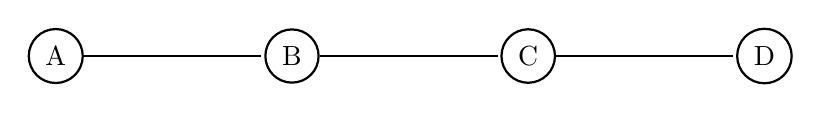
\begin{tikzpicture}[-,>=stealth',shorten >=1pt,auto,node distance=3cm, thick,main node/.style={circle,draw}, every loop/.style={}, scale=0.7]
            \node[main node] (A) {A};
            \node[main node] (B) [right of=A] {B};
            \node[main node] (C) [right of=B] {C};
            \node[main node] (D) [right of=C] {D};
            \path[every node/.style={font=\sffamily\small}]
            (A) edge node {} (B)
            (B) edge node {} (C)
            (C) edge node {} (D);
        \end{tikzpicture}}
        \end{center}

          \item \textbf{Bus Network}: All nodes are connected to a common medium along this medium. 

        \item \textbf{Star Network}: all nodes are connected to a special central node.
          \begin{center}
          \resizebox{3cm}{3cm}{%
          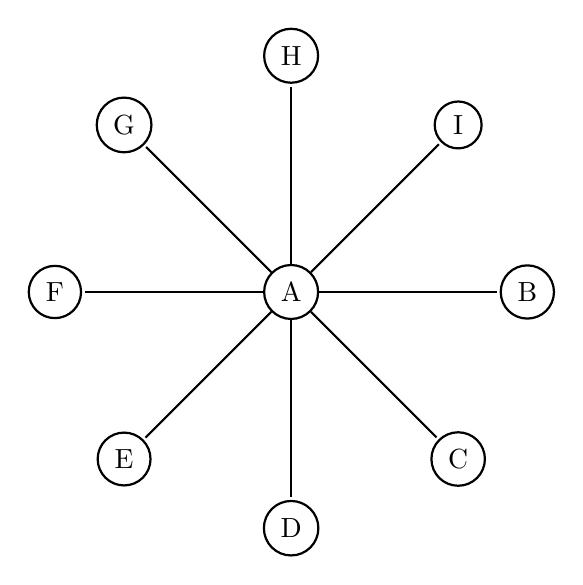
\begin{tikzpicture}[-,>=stealth',shorten >=1pt,auto,node distance=3cm, thick,main node/.style={circle,draw}, every loop/.style={}]
              \node[main node] (A) {A};
              \node[main node] (B) [right of=A] {B};
              \node[main node] (C) [below right of=A] {C};
              \node[main node] (D) [below of=A] {D};
              \node[main node] (E) [below left of=A] {E};
              \node[main node] (F) [left of=A] {F};
              \node[main node] (G) [above left of=A] {G};
              \node[main node] (H) [above of=A] {H};
              \node[main node] (I) [above right of=A] {I};
              \path[every node/.style={font=\sffamily\small}]
              (A) edge node {} (B)
              (A) edge node {} (C)
              (A) edge node {} (D)
              (A) edge node {} (E)
              (A) edge node {} (F)
              (A) edge node {} (G)
              (A) edge node {} (H)
              (A) edge node {} (I);
          \end{tikzpicture}}
          \end{center}

        \item \textbf{Ring Network}: Each node is connected to its left and right neighbour node, such that all nodes are connected and that each node can reach each other node by traversing nodes left- or rightwards.
          \begin{center}
          \resizebox{3cm}{3cm}{%
          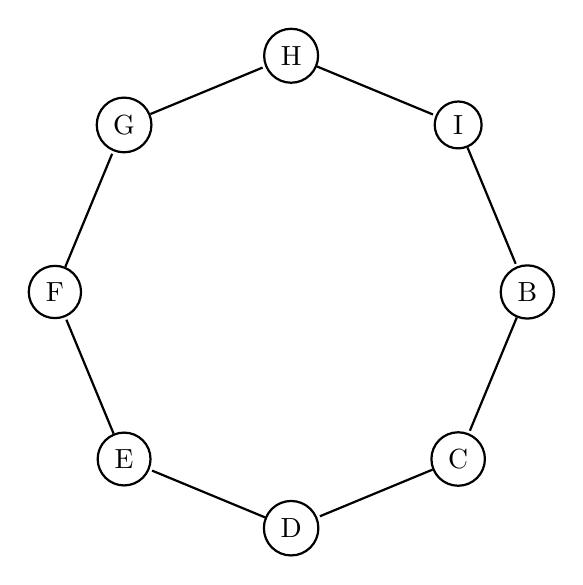
\begin{tikzpicture}[-,>=stealth',shorten >=1pt,auto,node distance=3cm, thick,main node/.style={circle,draw}, every loop/.style={}]
              \node[main node] (A) {A};
              \draw[white, fill=white] (-1,-1) rectangle (1,1);
              \node[main node] (B) [right of=A] {B};
              \node[main node] (C) [below right of=A] {C};
              \node[main node] (D) [below of=A] {D};
              \node[main node] (E) [below left of=A] {E};
              \node[main node] (F) [left of=A] {F};
              \node[main node] (G) [above left of=A] {G};
              \node[main node] (H) [above of=A] {H};
              \node[main node] (I) [above right of=A] {I};
              \path[every node/.style={font=\sffamily\small}]
              (B) edge node {} (C)
              (C) edge node {} (D)
              (D) edge node {} (E)
              (E) edge node {} (F)
              (F) edge node {} (G)
              (G) edge node {} (H)
              (H) edge node {} (I)
              (I) edge node {} (B);
          \end{tikzpicture}}
          \end{center}

        \item \textbf{Mesh Network}: each node is connected to an arbitrary number of neighbours in such a way that there is at least one traversal from any node to any other. 
          \begin{center}
          \resizebox{3.5cm}{3cm}{%
          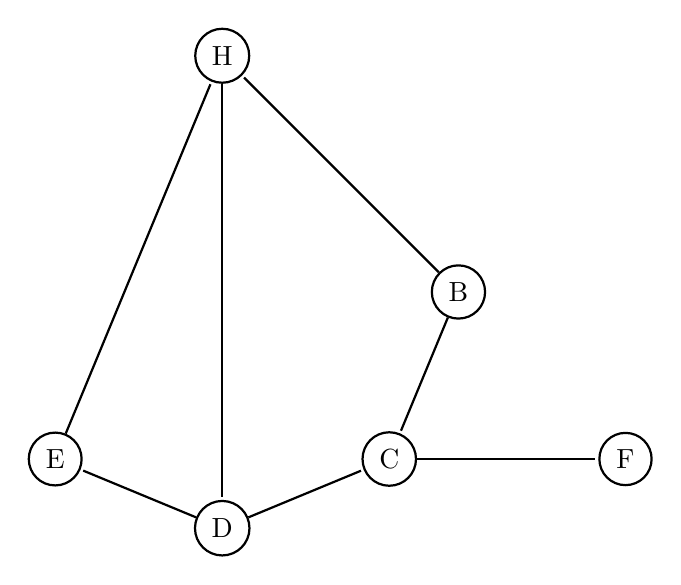
\begin{tikzpicture}[-,>=stealth',shorten >=1pt,auto,node distance=3cm, thick,main node/.style={circle,draw}, every loop/.style={}]
              \node[main node] (A) {A};
              \draw[white, fill=white] (-1,-1) rectangle (1,1);
              \node[main node] (B) [right of=A] {B};
              \node[main node] (C) [below right of=A] {C};
              \node[main node] (D) [below of=A] {D};
              \node[main node] (E) [below left of=A] {E};
              \node[main node] (H) [above of=A] {H};
              \node[main node] (F) [right of=C] {F};
              \path[every node/.style={font=\sffamily\small}]
              (B) edge node {} (C)
              (B) edge node {} (H)
              (D) edge node {} (C)
              (D) edge node {} (E)
              (C) edge node {} (F)
              (E) edge node {} (H)
              (H) edge node {} (D);
          \end{tikzpicture}}
          \end{center}

        \item \textbf{Fully Connected Network}: each node is connected to every other node in the network.
          \begin{center}
          \resizebox{3cm}{3cm}{%
          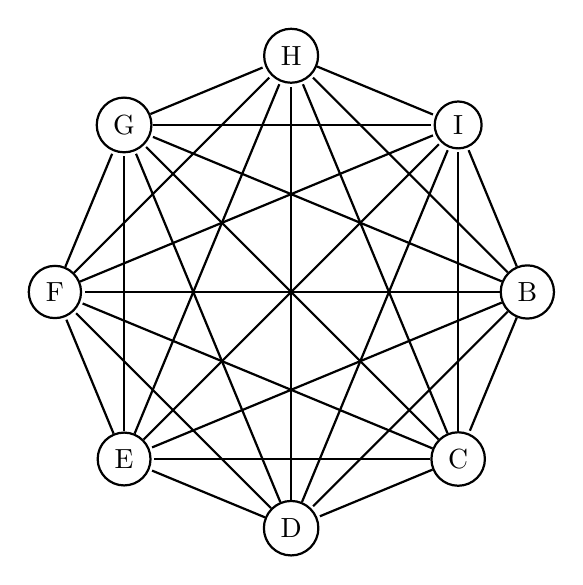
\begin{tikzpicture}[-,>=stealth',shorten >=1pt,auto,node distance=3cm, thick,main node/.style={circle,draw}, every loop/.style={}]
              \node[main node] (A) {A};
              \draw[white, fill=white] (-1,-1) rectangle (1,1);
              \node[main node] (B) [right of=A] {B};
              \node[main node] (C) [below right of=A] {C};
              \node[main node] (D) [below of=A] {D};
              \node[main node] (E) [below left of=A] {E};
              \node[main node] (F) [left of=A] {F};
              \node[main node] (G) [above left of=A] {G};
              \node[main node] (H) [above of=A] {H};
              \node[main node] (I) [above right of=A] {I};
              \path[every node/.style={font=\sffamily\small}]
              (B) edge node {} (C)
              (B) edge node {} (D)
              (B) edge node {} (E)
              (B) edge node {} (F)
              (B) edge node {} (G)
              (B) edge node {} (H)
              (B) edge node {} (I)
              (C) edge node {} (D)
              (C) edge node {} (E)
              (C) edge node {} (F)
              (C) edge node {} (G)
              (C) edge node {} (H)
              (C) edge node {} (I)
              (D) edge node {} (E)
              (D) edge node {} (F)
              (D) edge node {} (G)
              (D) edge node {} (H)
              (D) edge node {} (I)
              (E) edge node {} (F)
              (E) edge node {} (G)
              (E) edge node {} (H)
              (E) edge node {} (I)
              (F) edge node {} (G)
              (F) edge node {} (H)
              (F) edge node {} (I)
              (G) edge node {} (H)
              (G) edge node {} (I)
              (H) edge node {} (I);
          \end{tikzpicture}}
          \end{center}

        \item \textbf{Tree Network}: nodes are arranged hierarchically.
          \begin{center}
          \resizebox{5cm}{3cm}{%
          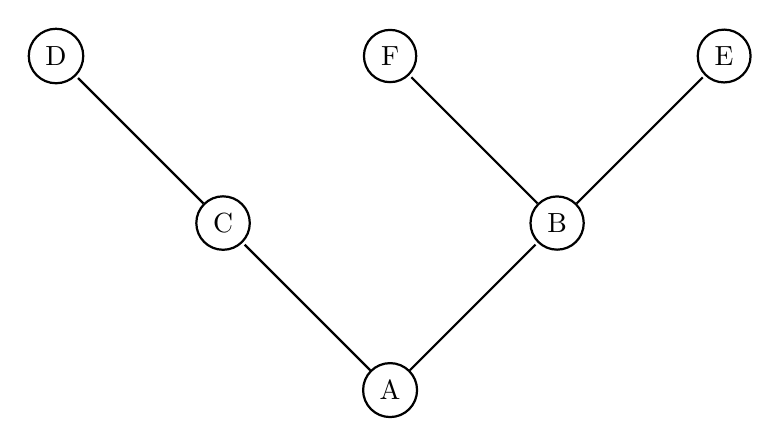
\begin{tikzpicture}[-,>=stealth',shorten >=1pt,auto,node distance=3cm, thick,main node/.style={circle,draw}, every loop/.style={}]
              \node[main node] (A) {A};
              \node[main node] (B) [above right of=A] {B};
              \node[main node] (C) [above left of=A] {C};
              \node[main node] (D) [above left of=C] {D};
              \node[main node] (E) [above right of=B] {E};
              \node[main node] (F) [above left of=B] {F};
              \path[every node/.style={font=\sffamily\small}]
              (A) edge node {} (B)
              (A) edge node {} (C)
              (B) edge node {} (F)
              (B) edge node {} (E)
              (C) edge node {} (D);
          \end{tikzpicture}}
          \end{center}
      \end{enumerate} 
    \end{example}

    Notice how many of these networks have \textbf{redundancy}: having multiple ways to get from one node to another. That is, when a network path is no longer available, data is still able to reach its destination through another path. Usually, we would like to avoid a \textbf{single point of failure} and construct a \textbf{fault-tolerant} system that can experience failure in its components but still continue operating properly. However, building more connections may be expensive. 

    Because there are multiple paths that a piece of data takes to get from point X to point Y, \textit{routing strategies} are implemented in order to determine the most optimal path. Now in order for network nodes to communicate with each other, they should have some sort of universal method of communicating with each other. 

    \begin{definition}[Communication Protocol]
      A \textbf{communication protocol} is a system of rules that allow multiple entities of a communications to transmit information via any kind variation of a physical quantity. The protocol defines the rules, syntax, semantics and synchronization of communication and possible error recovery methods. A protocol can have many jobs, such as: 
      
      \begin{enumerate} 
        \item Determining how nodes will communicate with each other . 
        \item Making sure that these modes of communication is compatible with hardware .
        \item Implementing security protocols such as encryption schemes. 
      \end{enumerate}
    \end{definition}

    Computers can connect through \textbf{physical} (e.g. cables) or \textbf{wireless} connections. 

    \begin{enumerate}
      \item The \textbf{CAT5 cable} is a \textit{twisted pair (copper) cable} that's designed for use in computer networks. It consists of four twisted pairs of copper wires. These twisted pair cables send data through a network by transmitting pulses of electricity that represent binary data. The information transmission follow the \textbf{Ethernet} standards, which is why twisted pair cables are commonly known as Ethernet cables. Use for both LANs and WANs. They can carry up to 1 Gbps across hundreds of feet, but are susceptible to interference. 

      \item \textbf{Fiber-optic cables} carry light instead of electricity in a fiber coated with plastic layers. The pulses of light represent binary data and also follow the Ethernet standards. They are also capable of transmitting much more data per second that copper cables, and they have the advantage of low transmission loss and immunity to electrical interference. Often used to connect networks across oceans so that data can travel quickly around the world. They can carry up to 26 Tbps acorss 50 miles (but are expensive)

      \item A wireless card inside a computer turns binary data into \textbf{radio waves} and transmits them through the air. However, they do not travel very far (~100 ft in office buildings or up to 1000 ft in an open field). The waves are picked up by a \textit{wireless access point} which converts them from radio waves back into binary data. These access points would be connected to the rest of the network using physical wiring. They can carry up to 1.3 Gbps. 

      \item \textbf{Infrared signals} and \textbf{microwaves} are sometimes used. 
    \end{enumerate}


    In order for the computers to send data into binary, they must convert this data into binary and send them as streams of 1s and 0s in a process called \textbf{line coding}. Furthermore, computers can raise efficiency of each wire by sending changing electric currents through a single wire. For example, rather than using three wires to encode $\texttt{101}$ as 

    \begin{center}
      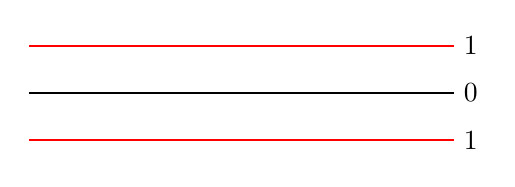
\begin{tikzpicture}[scale=0.6]
        \draw[thick, red] (0,1)--(9,1);
        \draw[thick] (0,0)--(9,0);
        \draw[thick, red] (0,-1)--(9,-1);
        \node[right] at (9,1) {1};
        \node[right] at (9,0) {0}; 
        \node[right] at (9,-1) {1};
      \end{tikzpicture}
    \end{center}

    they send it through a single wire with intervals of $\frac{1}{3}$ seconds

    \begin{center}
      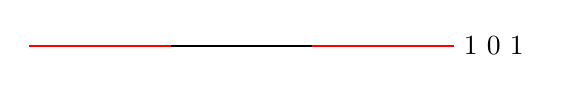
\begin{tikzpicture}[scale=0.6]
        \draw[thick, red] (0,0)--(3,0);
        \draw[thick] (3,0)--(6,0);
        \draw[thick, red] (6,0)--(9,0);
        \node[right] at (9,0) {1 0 1};
      \end{tikzpicture}
    \end{center}

    or even better, at a rate of 1 megabit per second (interval of $0.000001$ seconds)

    \begin{center}
      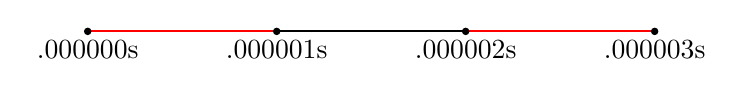
\begin{tikzpicture}[scale=0.8]
        \draw[thick, red] (0,0)--(3,0);
        \draw[thick] (3,0)--(6,0);
        \draw[thick, red] (6,0)--(9,0);
        \draw[fill] (0,0) circle (0.05);
        \draw[fill] (3,0) circle (0.05);
        \draw[fill] (6,0) circle (0.05);
        \draw[fill] (9,0) circle (0.05);
        \node[below] at (0,0) {.000000s};
        \node[below] at (3,0) {.000001s};
        \node[below] at (6,0) {.000002s};
        \node[below] at (9,0) {.000003s};
      \end{tikzpicture}
    \end{center}

    As long as two computers agree on the time period in which the electricity intervals are being sent, they can communicate much more efficiently. In an electrical connection (such as Ethernet), the signal would be a voltage or current. In an optical connection (such as a fiber-optic cable), the signal would be the intensity of light. 

    \begin{definition}
      There are many properties about line coding that are relevant, but ultimately the speed of a connection is a combination of the bandwidth and latency. 

      \begin{enumerate}
        \item The \textbf{bit rate} describes the data transfer rate of a connection. It measures the number of bit states that a channel can \textit{transmit} per unit time. It is measured in \textit{bits per second}. We can interpret it as the amount of water flowing through a pipe. 
        
        Bit rate is typically seen in terms of the actual data rate. But for most transmissions, the data represents part of a more complex protocol, which includes bits representing source address, destination address, error detection/correction codes, and other information. This data is called the \textbf{overhead}, while the actual data transferred is called the \textbf{payload}. At times, the overhead may be substantial (up to 20\% to 50\%). 

        \item The \textbf{throughput} is the number of bit states of usable information, that can be successfully \textit{received} over a channel per unit time. Without any channel noise, it is really just the payload. Note that this is an \textit{observed, dynamic parameter} with a fixed and variable loss. It is also known as \textbf{consumed bandwidth} and is measured in \textit{bits per second}. 
        
        \item The \textbf{bandwidth} describes the \textit{maximum} data transfer rate of a connection; that is, the maximum throughput of a communication. It is measured in \textit{bits per second}. We can interpret it as how thick the pipe is (i.e. how much water can flow through it at max). Note that this is different from the bandwidth used in signal processing. 
        
        Data often flows over multiple network connections, which means the connection with the smallest bandwidth (most likely your local connection) acts as a bottleneck. 
        
        \item The \textbf{latency}, or \textbf{ping-rate}, measures the round trip time between the sending of a data message to a computer and the receiving of that message, measured in \textit{milliseconds}. We can interpret it as the speed at which the water is flowing through a pipe. We can check latency by doing
        \begin{lstlisting}
          >>>ping www.google.com
          64 bytes: icmp_seq=0 ttl=115 time=37.868 ms
        \end{lstlisting}

        which outputs a latency time of 37.868ms (to get to $\texttt{www.google.com}$ and back) for sending a data packet of 64 bytes. Note that there is an intrinsic limiting factor to latency: the speed of light, which is approximately 1 foot per nanosecond. In addition to distance, another limiting factor is the congestion in the network and the type of connection. 
      \end{enumerate}
    \end{definition}

    \begin{example}
    Given two computers connected by a wire that is configured to transfer 1000 bits per second, the bit rate would be 1 Kbps. However, if the channel has noise and demands retransmission of 10 bits out of every 1000 of the original transmission, then the throughput would be 990 bps. 

    Furthermore, the Ethernet frame can have as many as 1542 bytes. Say that there are 1500 bytes of payload and an overhead of 42 bytes. Then, the \textbf{protocol efficiency} would would be 
    \[\frac{\text{payload}}{\text{frame size}} = \frac{1500}{1542} = 0.9727 = 97.3\%\]
    \end{example}

    Typically, the actual line rate is stepped up by a factor influenced by the overhead to achieve an actual target net data rate. In One Gigabit Ethernet, the actual line rate is 1.25 Gbits/s to achieve a net payload throughput of 1 Gbit/s. In a 10-Gbit/s Ethernet system, gross data rate equals 10.3125 Gbits/s to achieve a true data rate of 10 Gbits/s. The net data rate also is referred to as the throughput, or payload rate, of effective data rate.

  \subsection{History of the Internet}

    IETF, ICANN, IANA, ISPs.  

    \begin{example}[ARPANET]
      The ARPANET was the precursor to the Internet, the network where Internet technology was first tested out. It was started in 1969 with four computers connected to each other. 

        \begin{center}\resizebox{5cm}{3cm}{%
        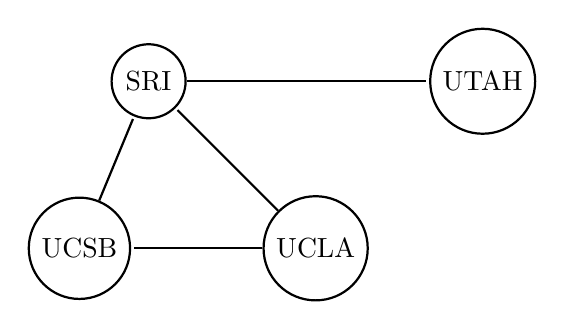
\begin{tikzpicture}[-,>=stealth',shorten >=1pt,auto,node distance=3cm, thick,main node/.style={circle,draw}, every loop/.style={}]
            \node[main node] (UCLA) {UCLA};
            \node[main node] (UCSB) [left of=UCLA] {UCSB};
            \node[main node] (SRI) [above left of=UCLA] {SRI};
            \node[main node] (UTAH) [above right of=UCLA] {UTAH};
            \path[every node/.style={font=\sffamily\small}]
            (UCLA) edge node {} (UCSB)
            (UCLA) edge node {} (SRI)
            (UCSB) edge node {} (SRI)
            (SRI) edge node {} (UTAH);
        \end{tikzpicture}}
        \end{center}

      For example, even if the path between SRI and UCSB is gone, the connections between SRI and UCSB is not lost (since IP packets can travel through UCLA's router). 
    \end{example}


    Now we can see an implementation of these networks in the internet. 

    \begin{definition}[Internet]
      The \textbf{Internet} is a global network of computing devices communicating with each other in some way, whether they're sending emails, downloading files, or sharing websites. The Internet is an \textbf{open network}, which means that any computing device can join as long as they follow the protocols. The internet is powered by many layers of protocols, and to create a global network of computing devices, we need: 

      \begin{enumerate}
        \item \textbf{Wires \& Wireless}: Physical connections between devices, plus protocols for converting electromagnetic signals into binary data. 
        \item \textbf{IP}: A protocol that uniquely identifies devices using IP addresses and provides a routing strategy to send data to a destination IP address. 
        \item \textbf{TCP/UDP}: Protocols that can transport packets of data from one device to another and check for errors along the way. 
        \item \textbf{TLS}: A secure protocol for sending encrypted data so that attackers can't view private information. 
        \item \textbf{HTTP \& DNS}: The protocols powering the World Wide Web
      \end{enumerate}        
    \end{definition}

    An \textbf{ISP (Internet Service Provider)} provides internet to its region. These ISPs are managed by certain continental autonomous systems (\textbf{AS}). The \textbf{Regional Internet Registry (RIR)} is divided into their regions: AFRNIC (Africa), ARIN (American), APNIC (Asia-Pacific), LACNIC (Latin America and Carribean), and RIPE NCC (European). 

    The main protocol suite used by the internet is \textbf{TCP/IP}, which is a collection of protocols that the internet uses. The bulk of this chapter will describe this protocol. 

    \begin{figure}[hbt!]
      \centering
      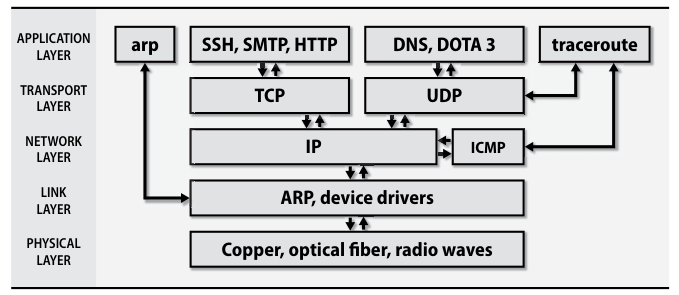
\includegraphics[scale=0.7]{img/tcp_ip_model.png}
      \caption{TCP/IP layering model. }
      \label{fig:tcp_ip_model}
    \end{figure}

  \subsection{Network Interfaces}

    Before we even start talking about IP addresses or protocols, we should mention that there are several interfaces from which computers can send and receive data. For example, if you are connected to both wired ethernet and WiFi, there are two paths, or interfaces, that data can travel. To see all your interfaces, use the \texttt{ip -c a} command. 

    \begin{lstlisting} 
      1: lo: <LOOPBACK,UP,LOWER_UP> mtu 65536 qdisc noqueue state UNKNOWN group default  
          link/loopback 00:00:00:00:00:00 brd 00:00:00:00:00:00
          inet 127.0.0.1/8 scope host lo
             valid_lft forever preferred_lft forever
          inet6 ::1/128 scope host noprefixroute 
             valid_lft forever preferred_lft forever
      2: wlan0: <BROADCAST,MULTICAST,UP,LOWER_UP> mtu 1500 qdisc noqueue state UP group 
          link/ether 64:bc:58:11:c0:24 brd ff:ff:ff:ff:ff:ff
          inet 10.197.221.245/16 brd 10.197.255.255 scope global dynamic noprefixroute 
             valid_lft 597085sec preferred_lft 597085sec
          inet6 fe80::b9e9:2f85:ded7:eaaf/64 scope link noprefixroute 
             valid_lft forever preferred_lft forever
    \end{lstlisting}

    The following lists out all the interfaces. We can see that we're connected to two interfaces, but there are a lot more. Usually, these interfaces also have a number following them that indexes different instances of the same type of interface. 

    \begin{enumerate} 
      \item \textbf{lo}: This is the loopback interface. 
      \item \textbf{wlan0}: For wireless connections 
      \item \textbf{tun}: When you are connected to VPN. 
      \item \textbf{en}: 
      \item \textbf{gif}: 
      \item \textbf{awd}: 
      \item \textbf{llw}: 
      \item \textbf{bridge}: 
      \item \textbf{utun}: 
    \end{enumerate}

    For each interface, there is a set of protocols that must be set for data to transfer. 

  \subsection{Addresses}

    Every computer needs some address that determines its unique identity. The version of TCP/IP that has been in widespread use is IPv4, which uses 4-byte IP addresses. A modernized version, IPv6, expands the IP address space to 16 bytes and incorporates several additional features, making it faster and easier to implement. 

    \begin{definition}[IP Address]
      The protocol describes the use of \textbf{IP addresses} to uniquely identify Internet-connected devices (for transmission of data). That is, when a computer sends a message to another computer, it must specify the recipient's IP address and also include its own IP address so that the second computer can reply. There are two versions of the Internet Protocol in use today: 
      \begin{enumerate}
          \item \textbf{IPv4}: The first version ever used on the Internet and having the form of 4 \textit{octets} split by periods in between. 

            \[[0-255].[0-255].[0-255].[0-255]\]

          Even though it presented in decimal, computers store them in binary 

            \[74.125.20.113 \iff 01001011.01111101.00010100.01110001\]

          IPv4 addresses can take $2^{32}$ values, but IPv6 was created for more space.

          \item \textbf{IPv6}: The newer standard (introduced in June 2012) is in the form 

            \[\text{FFFF:FFFF:FFFF:FFFF:FFFF:FFFF:FFFF:FFFF}\]

          with hexadecimal digits (total of ~$3.4 \times 10^{39}$ possible IPv6 values). 
      \end{enumerate}
    \end{definition}


    \begin{definition}[CIDR Notation]
      Sometimes, a set of IP addresses are specified using \textbf{CIDR notation}. An address of the form 

        \[145.201.67.4/16\]

      represents all addresses of form $145.201.\ast.\ast$. 
    \end{definition}

    Operating systems and network devices have supported IPv6 for a long time, and the motivation behind the deployment of IPv6 was due to the concern that devices were running out of IPv4 addresses. Asia ran out first in 2011, followed by every other continent ever since then. 

    But we've learned to make more efficient use of the IPv4 addresses that we have. For example, \textbf{Network Address Translation} (or \textbf{NAT}) lets entire networks of machines hide behind single IPv4 addresses. \textbf{Classless Inter-Domain Routing} (\textbf{CIDR}) subdivides networks and promotes efficient backbone routing as well. Ultimately, IPv6, with better security and engineering, is going to take over, but not for a while since it's not fundamentally different from IPv4 and the drawbacks of IPv4 haven't been bad enough to spark migration. 

    \begin{definition}[Hierarchy of IP Addresses] 
      The IP addresses are formatted in an \textit{hierarchical way}. The IPv4 address hierarchy is structured as such: The first few numbers (may or may not be divided by octets) could identify a \textbf{network} administered by an Internet Service Provider. The last numbers, which can also represent \textbf{subnetworks} (subnets), identifies a home computer on that network. 
    \end{definition}

    \begin{example}[University of Michigan]
      For example, if we represent the IP address 141.213.127.13 in binary (of 32 bits)

        \[10001101.11010101.01111111.00001101\]

      the first 16 bits could route to all of UMich, the next two bits could route to a specific UMich department, and the final 14 bits could route to individual computers. 
      \begin{center}
      \begin{tabular}{l|l|l}
          1000110111010101 & 01 & 11111100001101  \\
          \hline
          UMich Network & Medicine department & Lab computer 
      \end{tabular}
      \end{center}
      This hierarchy gives UMich the ability to differentiate between $2^2$ departments and $2^{14} = 16,384$ computers within each department. In general, the ability to create hierarchical levels at any point in the IP address allows for greater flexibility in the size of each level of the hierarchy. 
    \end{example}
    
    \begin{example}[Duke]
      Duke's IP addresses are of the form $153.3.\_.\_$, with the DUKE-INTERCHANGE ISP provider.  
    \end{example} 

    \begin{definition}[Hostname]
      IP addresses can be quite cumbersome to memorize, which is why they are often addressed with their \textbf{hostname}. Operating systems allow one or more hostnames to be associated with an IP address so that users can type \texttt{rfc-editor.org} rather than $4.31.198.49$. This mapping can be set up  in multiple days, e.g. with the \texttt{/etc/hosts} file or the LDAP database system to DNS the world-wide \textbf{Domain Name System}. 
    \end{definition}

    \subsubsection{LAN Addresses and NAT} 

      We've talked about how entire networks of machines can hide behind a single IPv4 address. Let's elaborate on this. In fact, your computer is not connected to the internet directly. It is actually in a \textbf{private network}, or a \textit{LAN network}, which uses a private IP address space (supported by both IPv4 and v6). Anything on the inside of your private network is not on the Internet; it is on your LAN, an entirely separate network, with its own address space. Anything on your LAN must have a unique (within the LAN) IP address to participate properly with your local network. Therefore, anyone else who has a LAN is also not part of the internet. So if you are only on your LAN network, how do you actually connect to the internet? 

      \begin{definition}[Router] 
        The \textbf{router} is a device that forms a connection between your LAN network and the internet. It has both a private local address, called a \textbf{gateway address}, and a public address. It is responsible for forwarding data between the local server computers and the internet. Therefore, to the outside world, all devices identify the network internet activity by the one public IP address assigned to the router. 

        The gateway address can be found with \texttt{ip route} and the public address, of course, can be found with the commands previously mentioned. 
      \end{definition}

      \begin{definition}[Modem]
        A \textbf{modem}, short for \textbf{modulator/demodulator} is a device that converts a signal from your computer to some kind of signal to talk to other computers. The main difference between the router and the modem is that 
        \begin{enumerate} 
           \item The router crates a network between the computers in your home and routes network traffic between them (through Ethernet cables or wireless connection). Your home router has one connection to the Internet and connections to your private local network. 

          \item The modem serves as a bridge between your local network and the Internet.  
        \end{enumerate}
      \end{definition}

      To access our IP address, we can do the following: 
      \begin{enumerate} 
        \item To access local ip address, we can either run the command \texttt{hostname -i}, \texttt{ip -c a}, or \texttt{ifconfig}.
          
        \item To access the public ip address, we can either google it or run \texttt{curl ifconfig.me}. Since this is public, any device connected to the same network/router should have the same IP address. 
      \end{enumerate}

      \begin{definition}[NAT]
        In order for LAN devices to connect to the Internet, their outgoing traffic has the source address changed to match that of the internet/WAN IP address of the router. The router keeps track of this, and makes sure any response traffic gets sent to the right internal machine. This is called \textbf{Network Address Translation (NAT)}. There are generally two types of NAT: 

        \begin{enumerate}
          \item \textbf{Basic, one-to-one NAT}: The simplest type of NAT provides a one-to-one translation of IP addresses. In this type of NAT, only the IP addresses, IP header checksum, and any higher-level checksums that include the IP address are changed. Basic NAT can be used to interconnect two IP networks that have incompatible addressing. 

          \item \textbf{One-to-many NAT}: The majority of network address translators map multiple private hosts to one publicly exposed IP address. In a typical configuration, a local network uses one of the designated private IP address subnets. A router in that network has a private address of that address pace. The router it also connected to the Internet with a \textit{public} address assigned by the ISP. As traffic passes from the local network to the Internet, the source address in each packet is translated on the fly from a private address to the public address. The router tracks basic data about each active connection (particularly the destination address and port). When a reply returns to the router, it uses the connection tracking data it stored during the outbound phase to determine the private address on the internal network to which to forward the reply. 
        \end{enumerate}
      \end{definition}

      \begin{definition}
        The IP addresses that are in the private network's space are usually divided up into 3 categories. But as of now, the categories don't mean anything. 

        \begin{enumerate}
          \item \textbf{Class A private range addresses}: 10.0.0.0 - 10.255.255.255 (16,777,216 IPs)
          \item \textbf{Class B private range addresses}: 172.16.0.0 – 172.31.255.255 (1,048,576 IPs)
          \item \textbf{Class C private range addresses}: 192.168.0.0 – 192.168.255.255 (65,536 IPs)
        \end{enumerate}

        Since the private IPv4 address space is relatively small, many private IPv4 networks unavoidably use the same address ranges. This can create a problem when merging such networks, as some addresses may be duplicated for multiple devices. In this case, networks or hosts must be renumbered, often a time-consuming task, or a network address translator must be placed between the networks to translate or masquerade one of the address ranges. 
      \end{definition}


    \subsubsection{Ports}

      IP addresses identify a machine's network interfaces, but they aren't specific enough to address individual processes or services, many of which might be actively using the network at once. TCP and UDP extend IP addresses with a concept known as a port, which is a 16-bit number that supplements an IP address to a particular communication channel. Valid ports range from $1$ to $65,535$. A port, combined with an IP address, results in a \textbf{socket address} that is used to establish a connection between a client and a server. 

      UNIX systems restrict programs from binding to port numbers under 1024 unless they are run as root or have an appropriate Linux capability. Anyone can communicate with a server running on a low port number; the restriction only applies to the program listening on the port.

    \subsubsection{Hardware (MAC) Addresses}

      The lowest level of addressing is the network hardware. Many devices are assigned a unique 6-byte hardware address at the time of manufacture. The first 3 bytes identify the manufacturer, and the last 3 bytes are a unique serial number that the manufacturer assigns. Sysadmins can sometimes identify the brand of machine that is trashing a network by looking up the 3-byte identifier in a table of vendor IDs. In theory, ethernet hardware addresses are permanently assigned and immutable, but many network interfaces let you override the hardware address and set one of your own choosing. 

  \subsection{TCP Packets and Encapsulation}

  \subsection{OSI and Internet Protocols}
  

  \subsection{HTTP and HTTPS} 

    HTTP stands for hypertext transfer protocol, implemented in Layer 7, which transfers data between your computer and the server over the internet through \textbf{clear text}. This may not be the most ideal way since any interceptors can read the transferred data. This isn't a problem for regular internet browsing, but if you are inputting sensitive data, then HTTP should not be used. This is why HTTPS (which stands for secure HTTP) was invented, which  is implemented in Layer 4 and encrypts the data being transferred, and every website where you input sensitive data should be using HTTPS (indicated by the \texttt{https://} prefix in the URL and a padlock symbol for modern browsers). Due to the extra security measures, HTTPS is less lightweight than HTTP, and its respective default ports are HTTP (80) and HTTPS (443).  

    A natural question to ask would be: which encryption scheme does HTTPS use? Both Secure Sockets Layer (SSL) and Transport Layer Security (TLS) is used in the modern web. 

    SSL certificate. 

    
  \subsection{UDP and TCP}

    TCP handshake can be seen with curl. 

\end{document}
